\documentclass[aspectratio=169]{beamer}
\setbeamertemplate{navigation symbols}{}
\usepackage{color, amsmath, comment, subfigure}
\usepackage{url}

\usepackage{hyperref}
\hypersetup{
    colorlinks=true,
    linkcolor=blue,
    filecolor=magenta,      
    urlcolor=cyan,
}

%%%%%%%%%%%%%%%%%%%%%%%%%%
\title[]{Class slides for Tuesday, October 6:\\Social fads, part 1}
\author[]{Matthew J. Salganik}
\institute[]{}
\date[]{COS 597E/SOC 555 Limits to prediction\\Fall 2020, Princeton University}

\begin{document}
%%%%%%%%%%%%%%%%%%%%%%%%%%%
\frame{\titlepage}
%%%%%%%%%%%%%%%%%%%%%%%%%%%
\begin{frame}

\begin{figure}
  \centering
  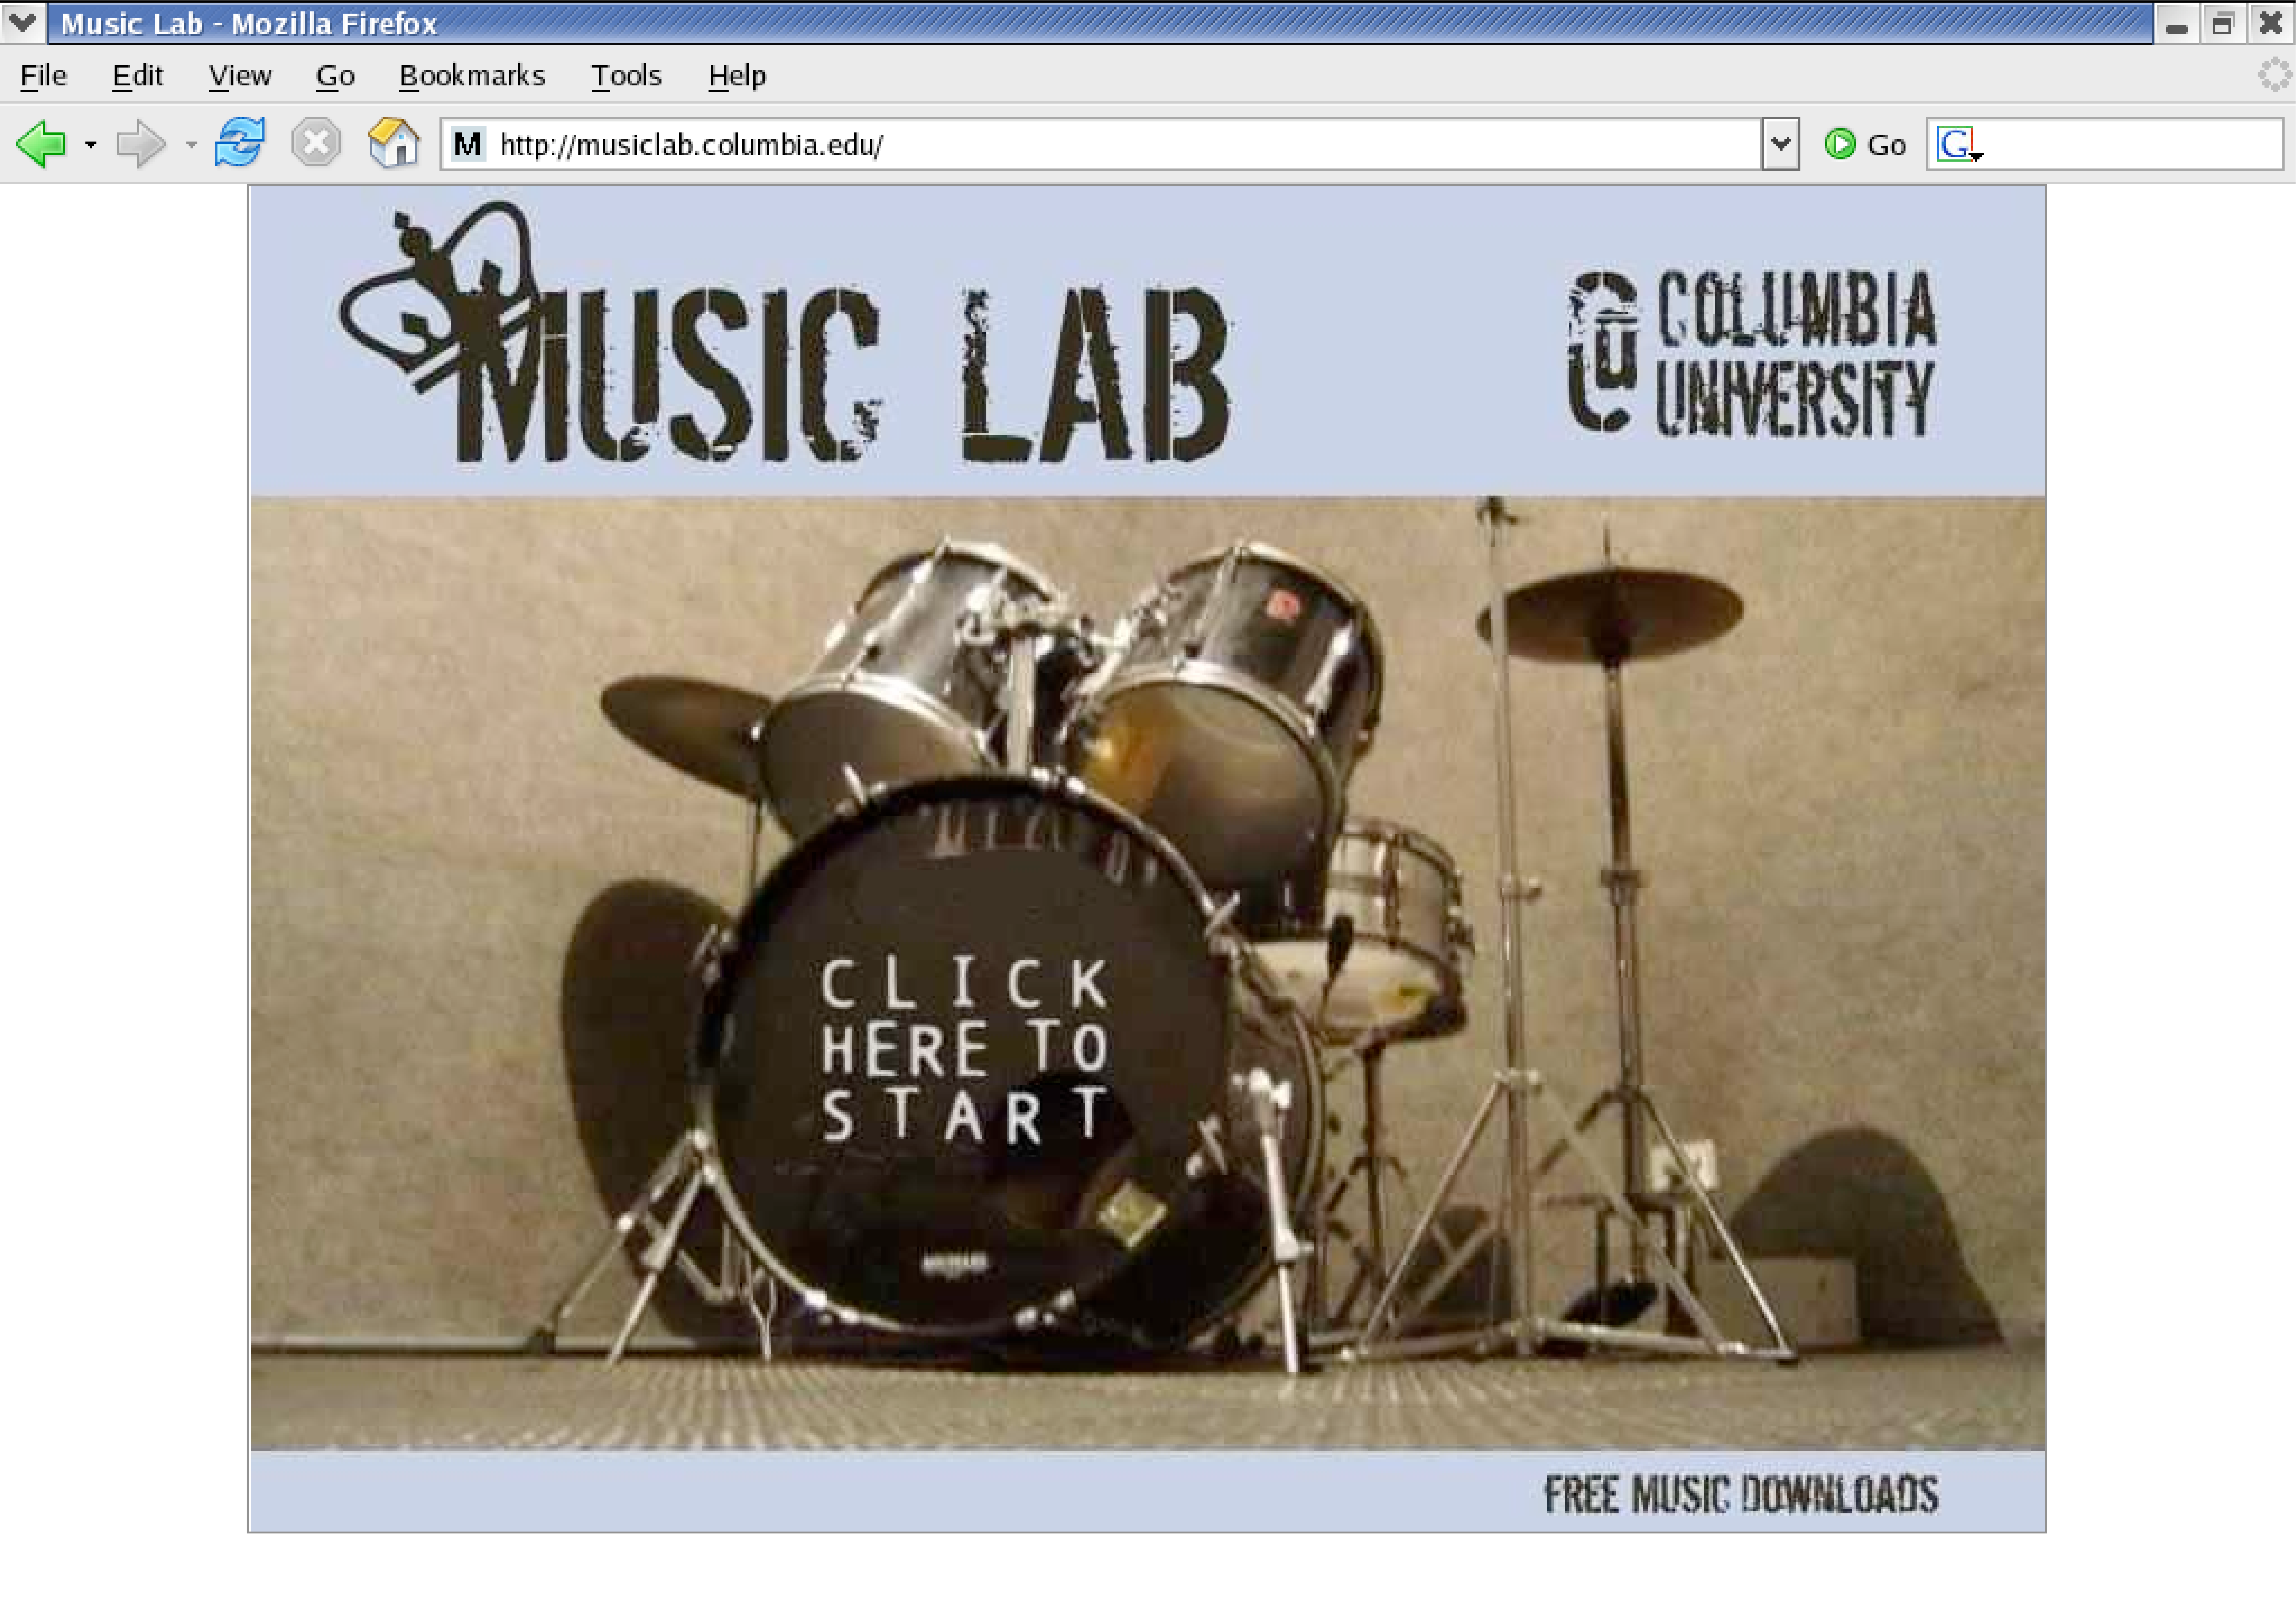
\includegraphics[width = 0.9\textwidth]{figures/splashscreen}
\end{figure}

\end{frame}
%%%%%%%%%%%%%%%%%%%%%%%%%%%%%%%%%
\begin{frame}

\begin{figure}
  \centering
  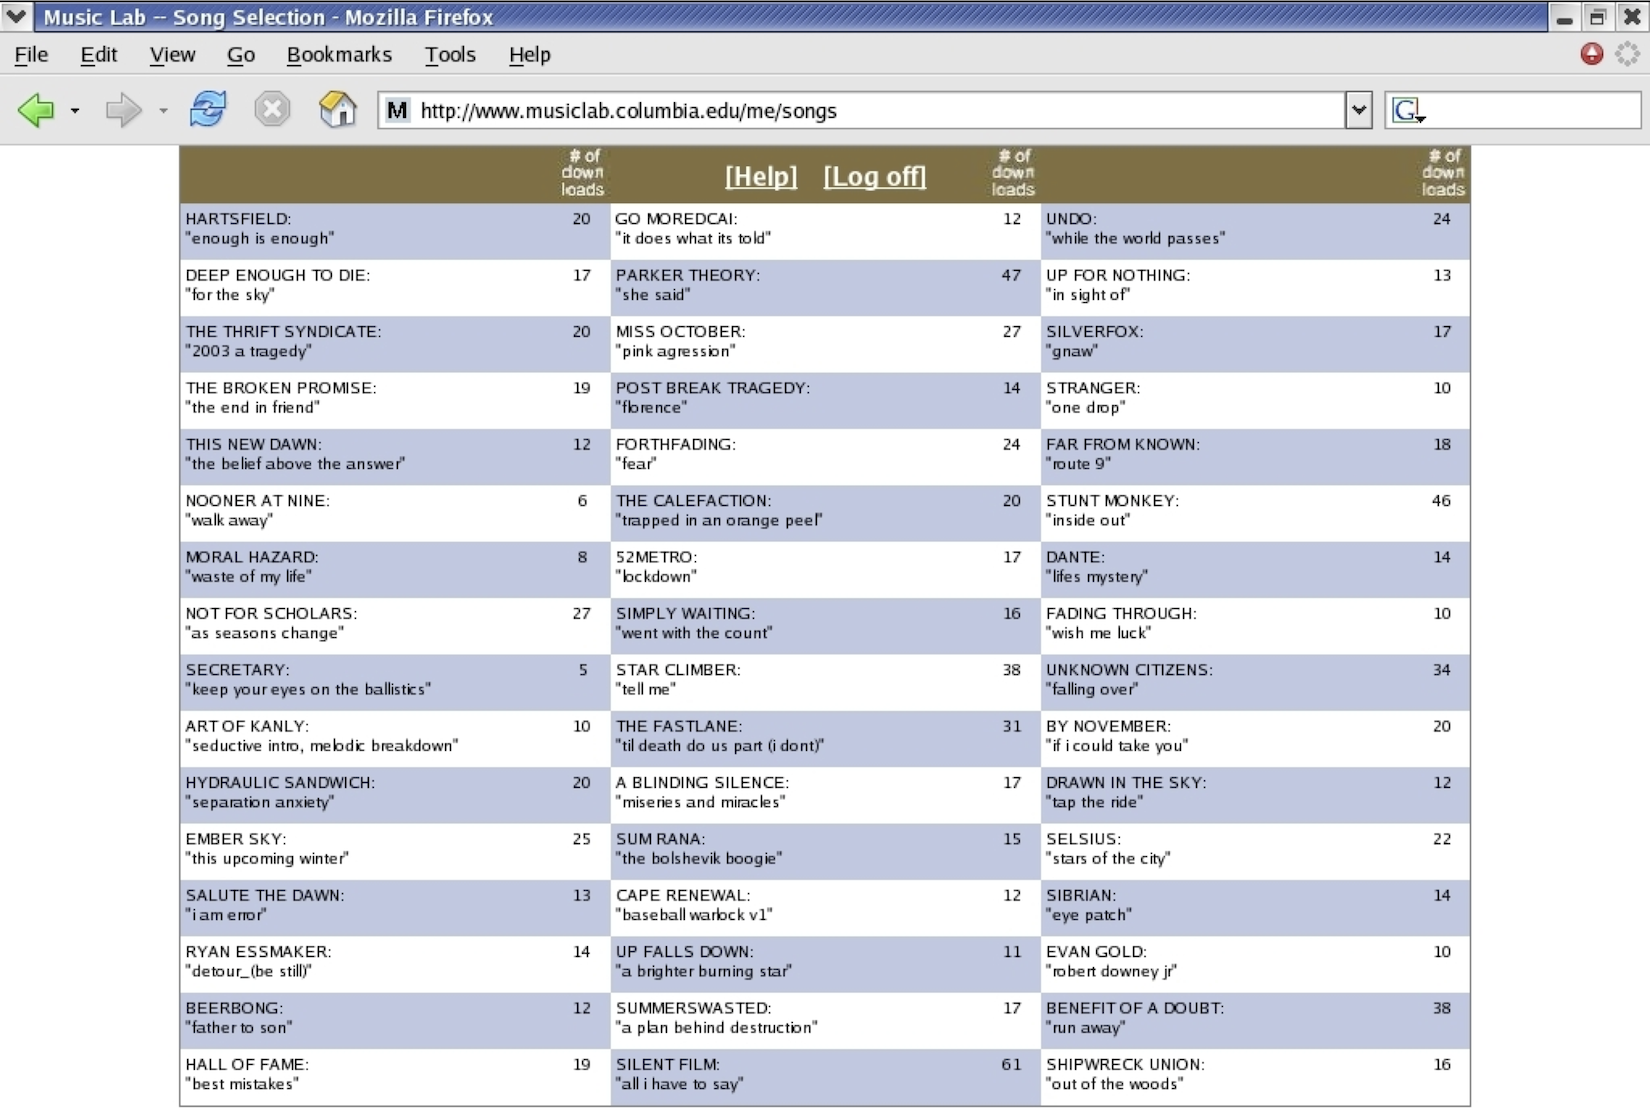
\includegraphics[width = 0.9\textwidth]{figures/info-v1-cut}
\end{figure}

\end{frame}
%%%%%%%%%%%%%%%%%%%%%%%%%%%%%%%%%
\begin{frame} 

\begin{figure}
  \centering
  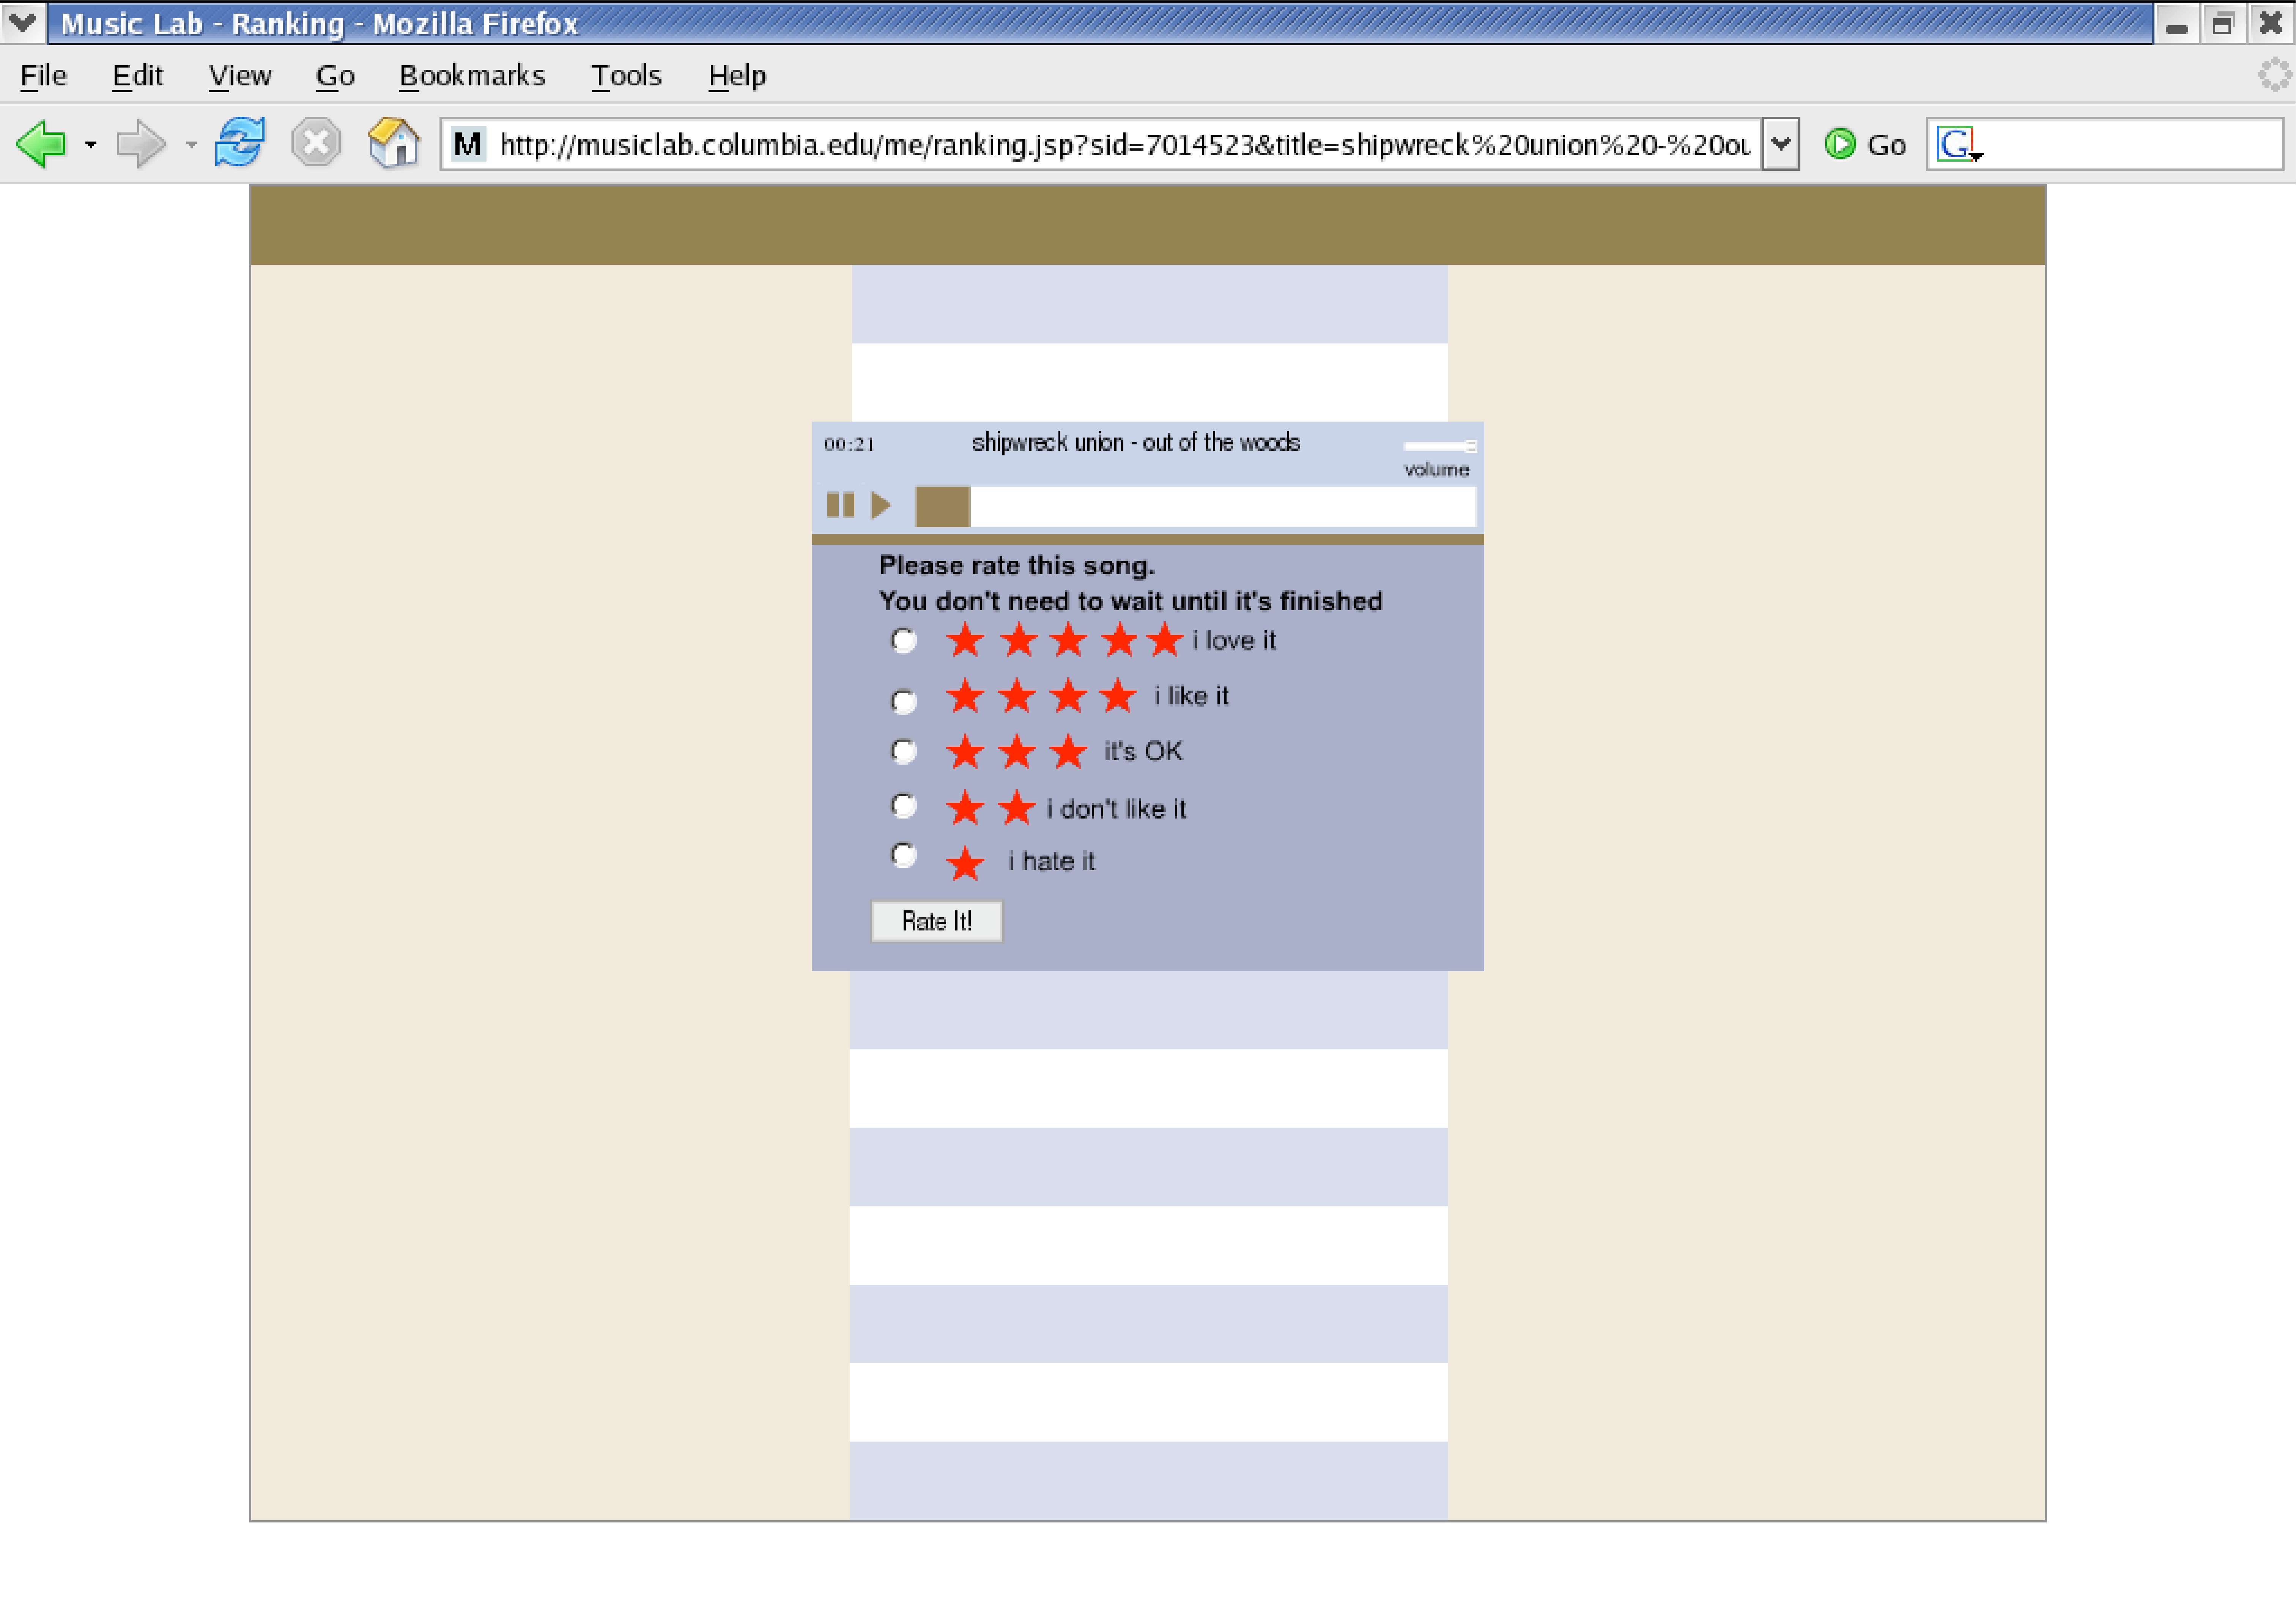
\includegraphics[width = 0.9\textwidth]{figures/listenscreen}
\end{figure}

\end{frame}
%%%%%%%%%%%%%%%%%%%%%%%%%%%%%%%%%
\begin{frame}

\begin{figure}
  \centering
  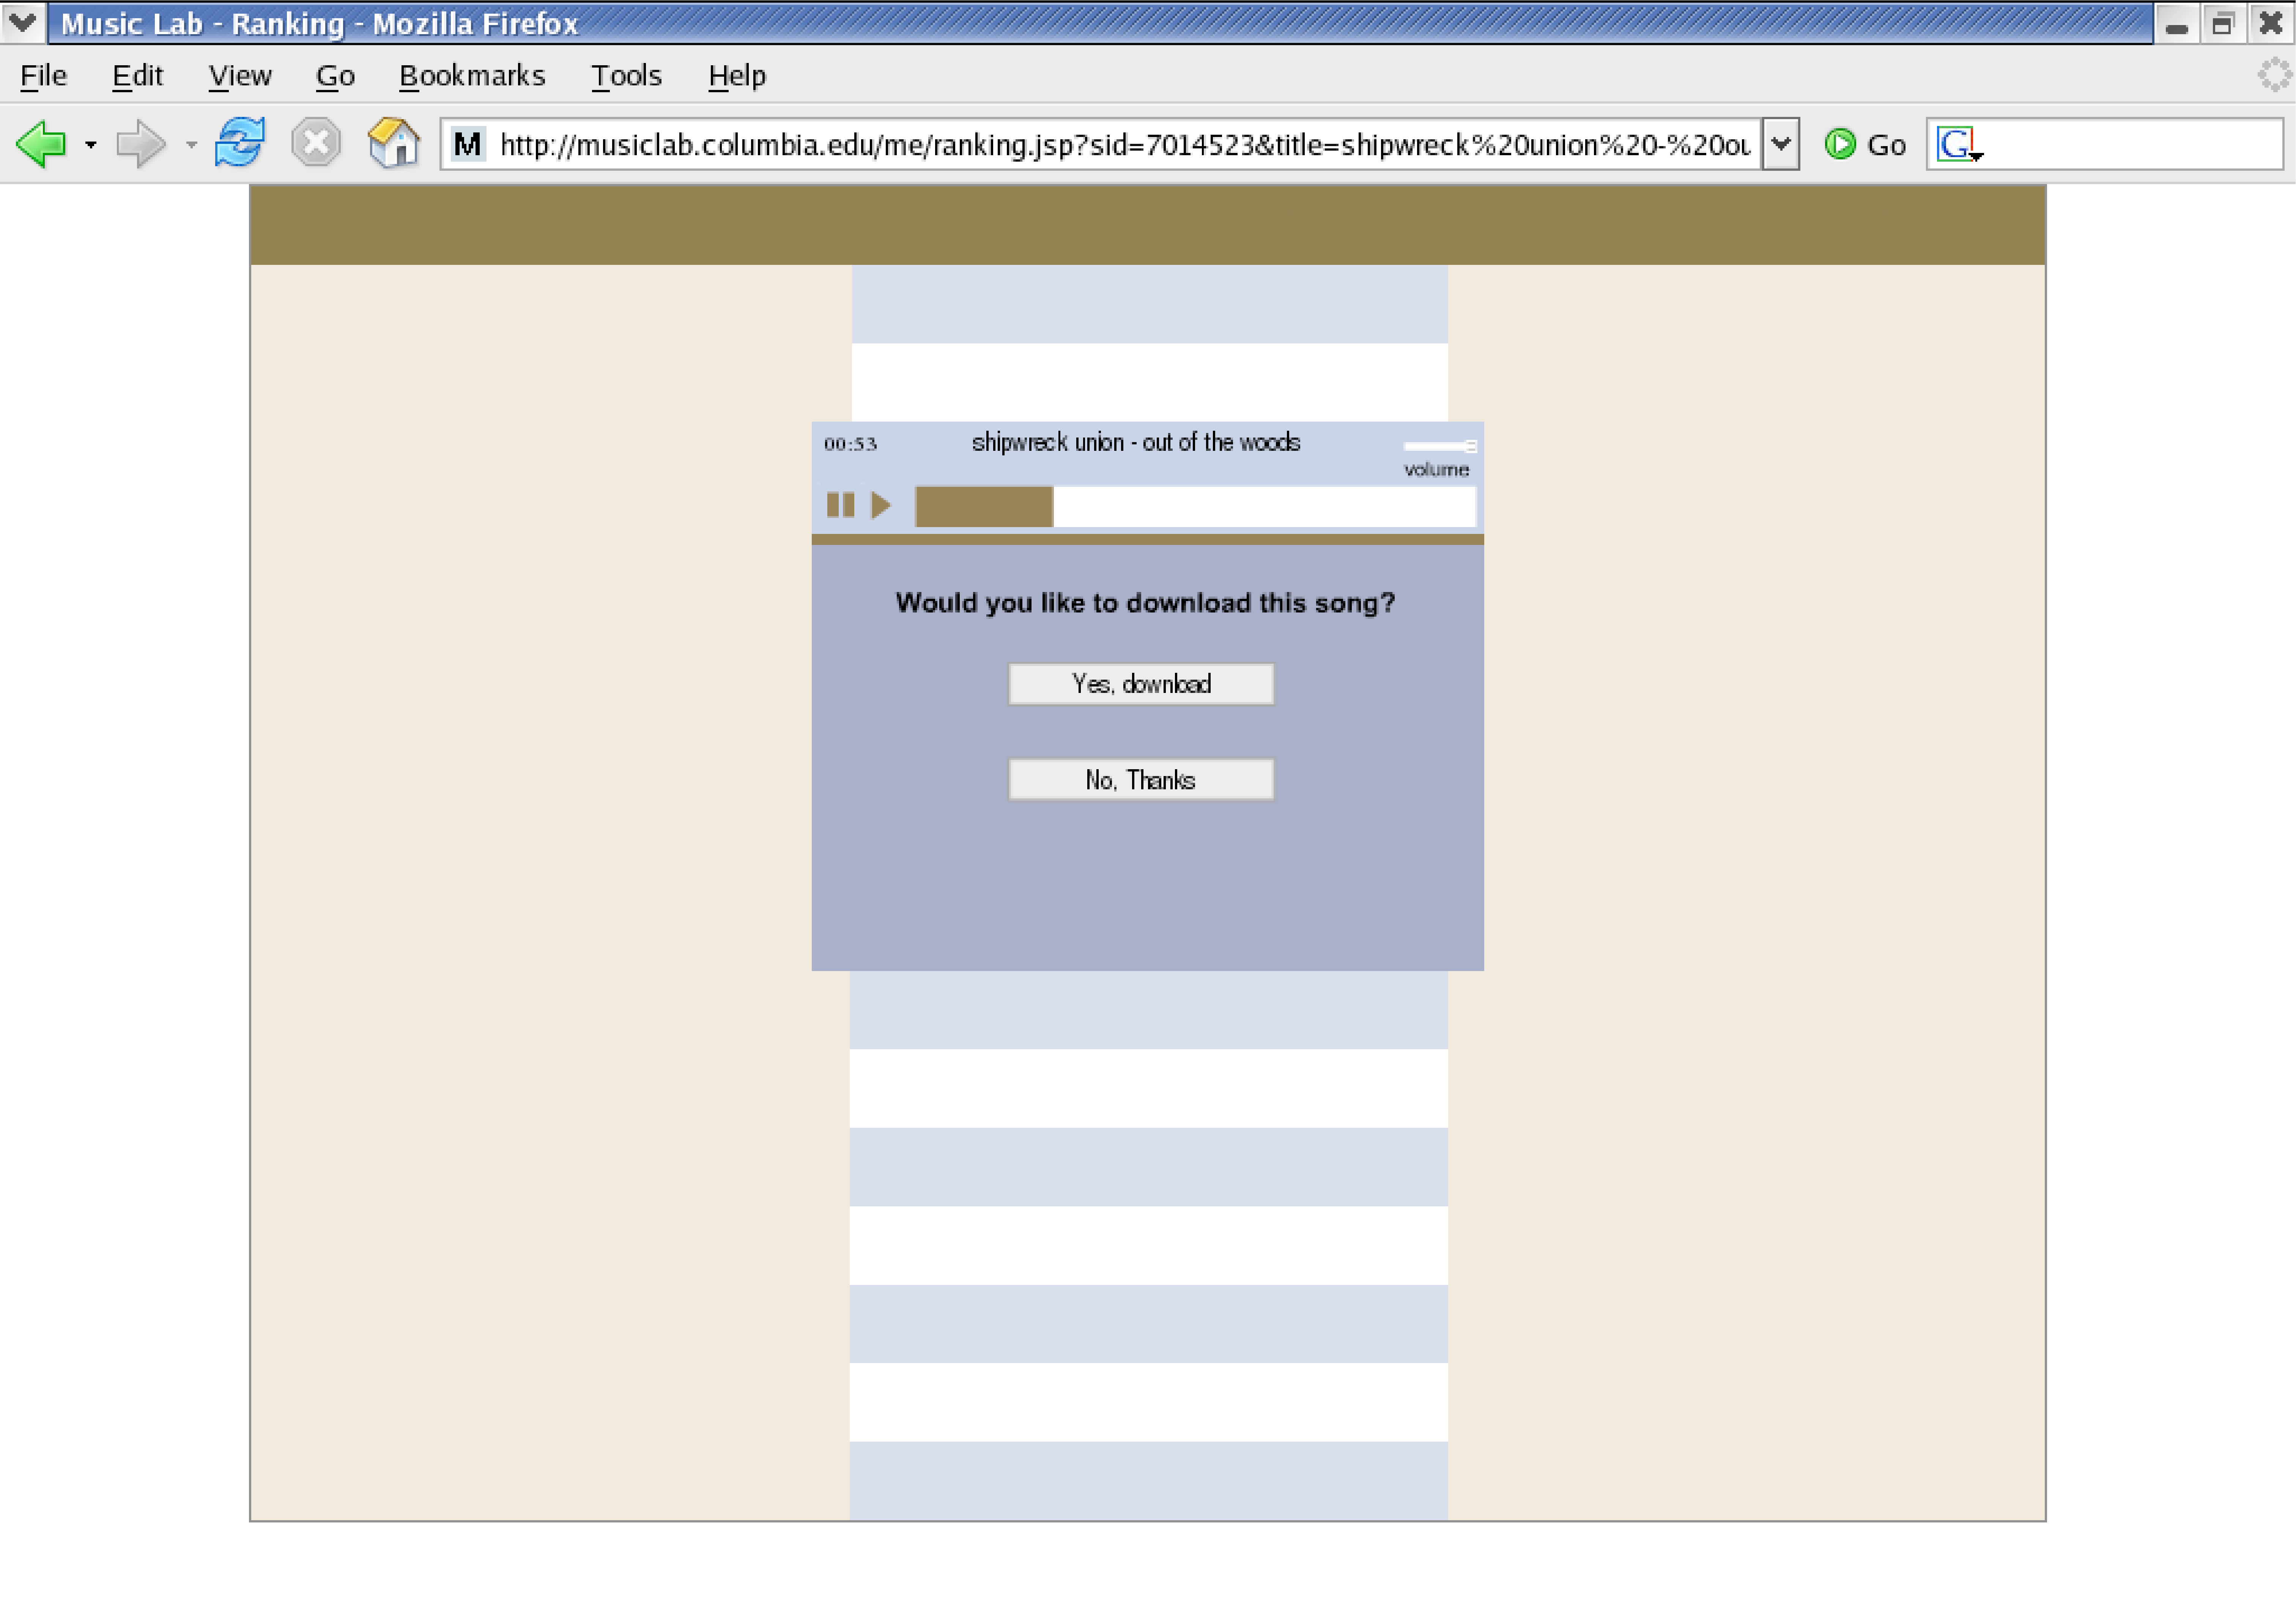
\includegraphics[width = 0.9\textwidth]{figures/downloadscreen}
\end{figure}

\end{frame}
%%%%%%%%%%%%%%%%%%%%%%%%%%%%%%%%%%
\begin{frame}

\begin{figure}
  \centering
  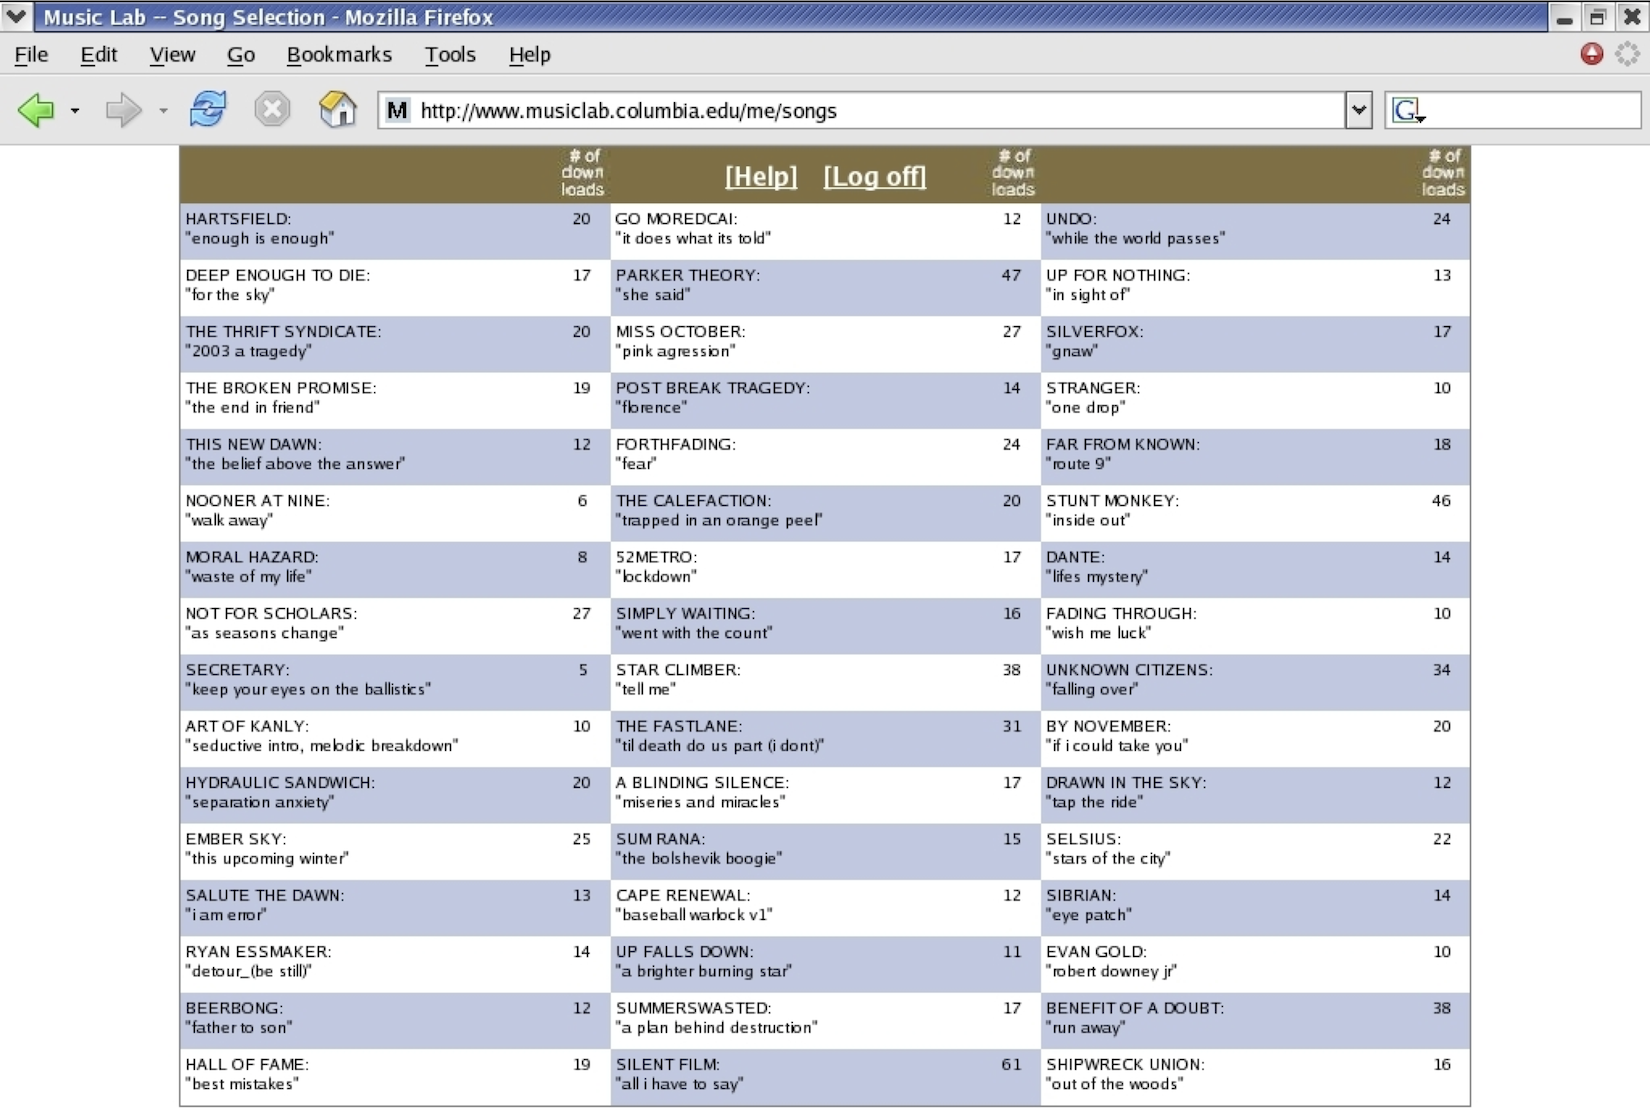
\includegraphics[width = 0.9\textwidth]{figures/info-v1-cut}
\end{figure}

\end{frame}
%%%%%%%%%%%%%%%%%%%%%%%%%%%%%%%%%
\begin{frame}

\begin{figure}
  \centering
  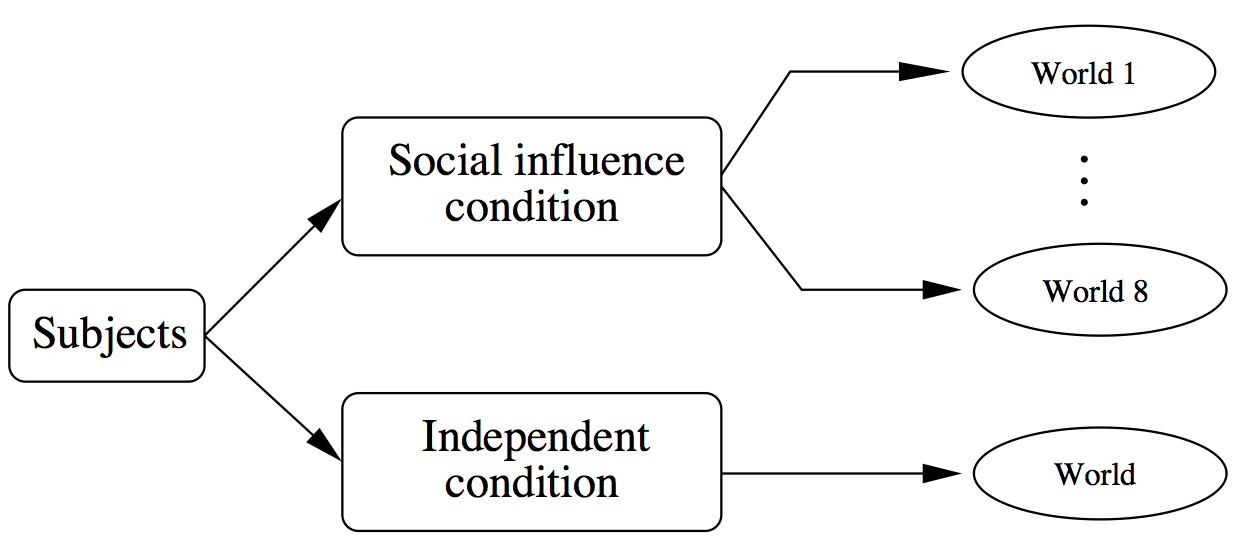
\includegraphics[width=0.9\textwidth]{figures/musiclab_exp_design}
\end{figure}

\end{frame}
%%%%%%%%%%%%%%%%%%%%%%%%%%%%%%%%%
\begin{frame}

\setcounter{subfigure}{0}
\begin{figure}
  \centering
     \subfigure[Experiment 1, Weaker signal]{
     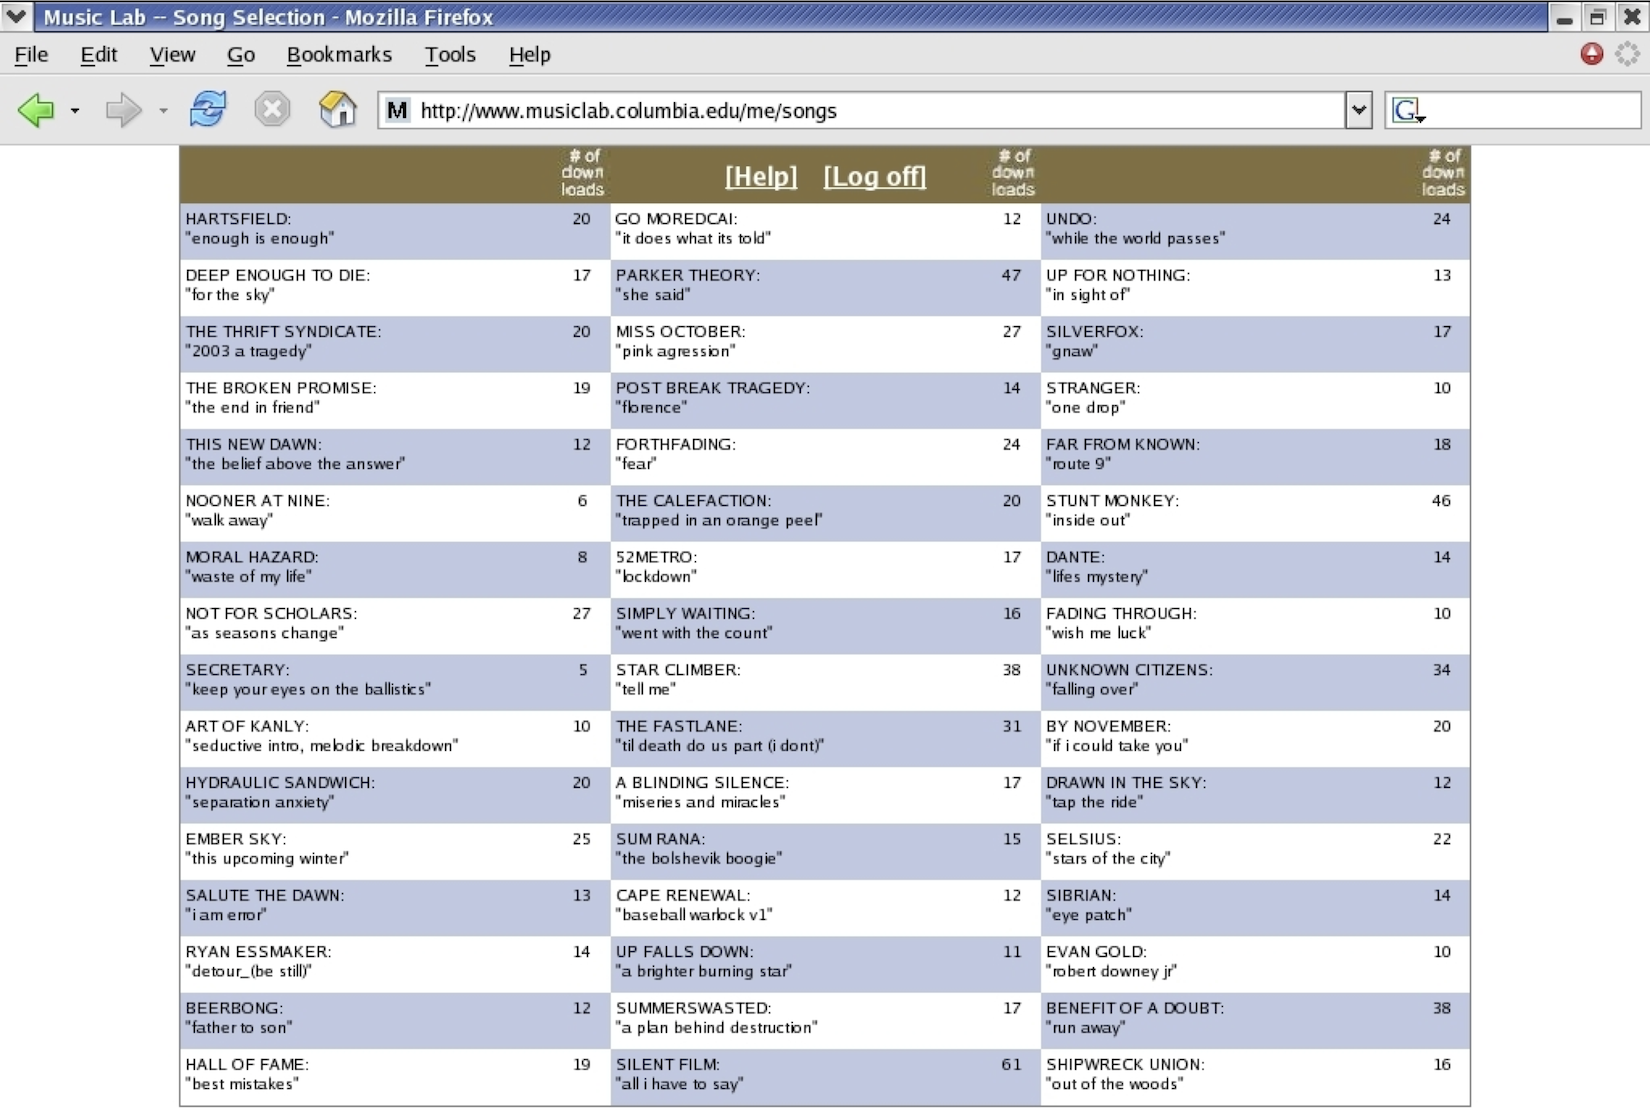
\includegraphics[width=0.45\textwidth]{figures/info-v1-cut}}
  \hspace{0in}
     \subfigure[Experiment 2, Stronger signal]{
     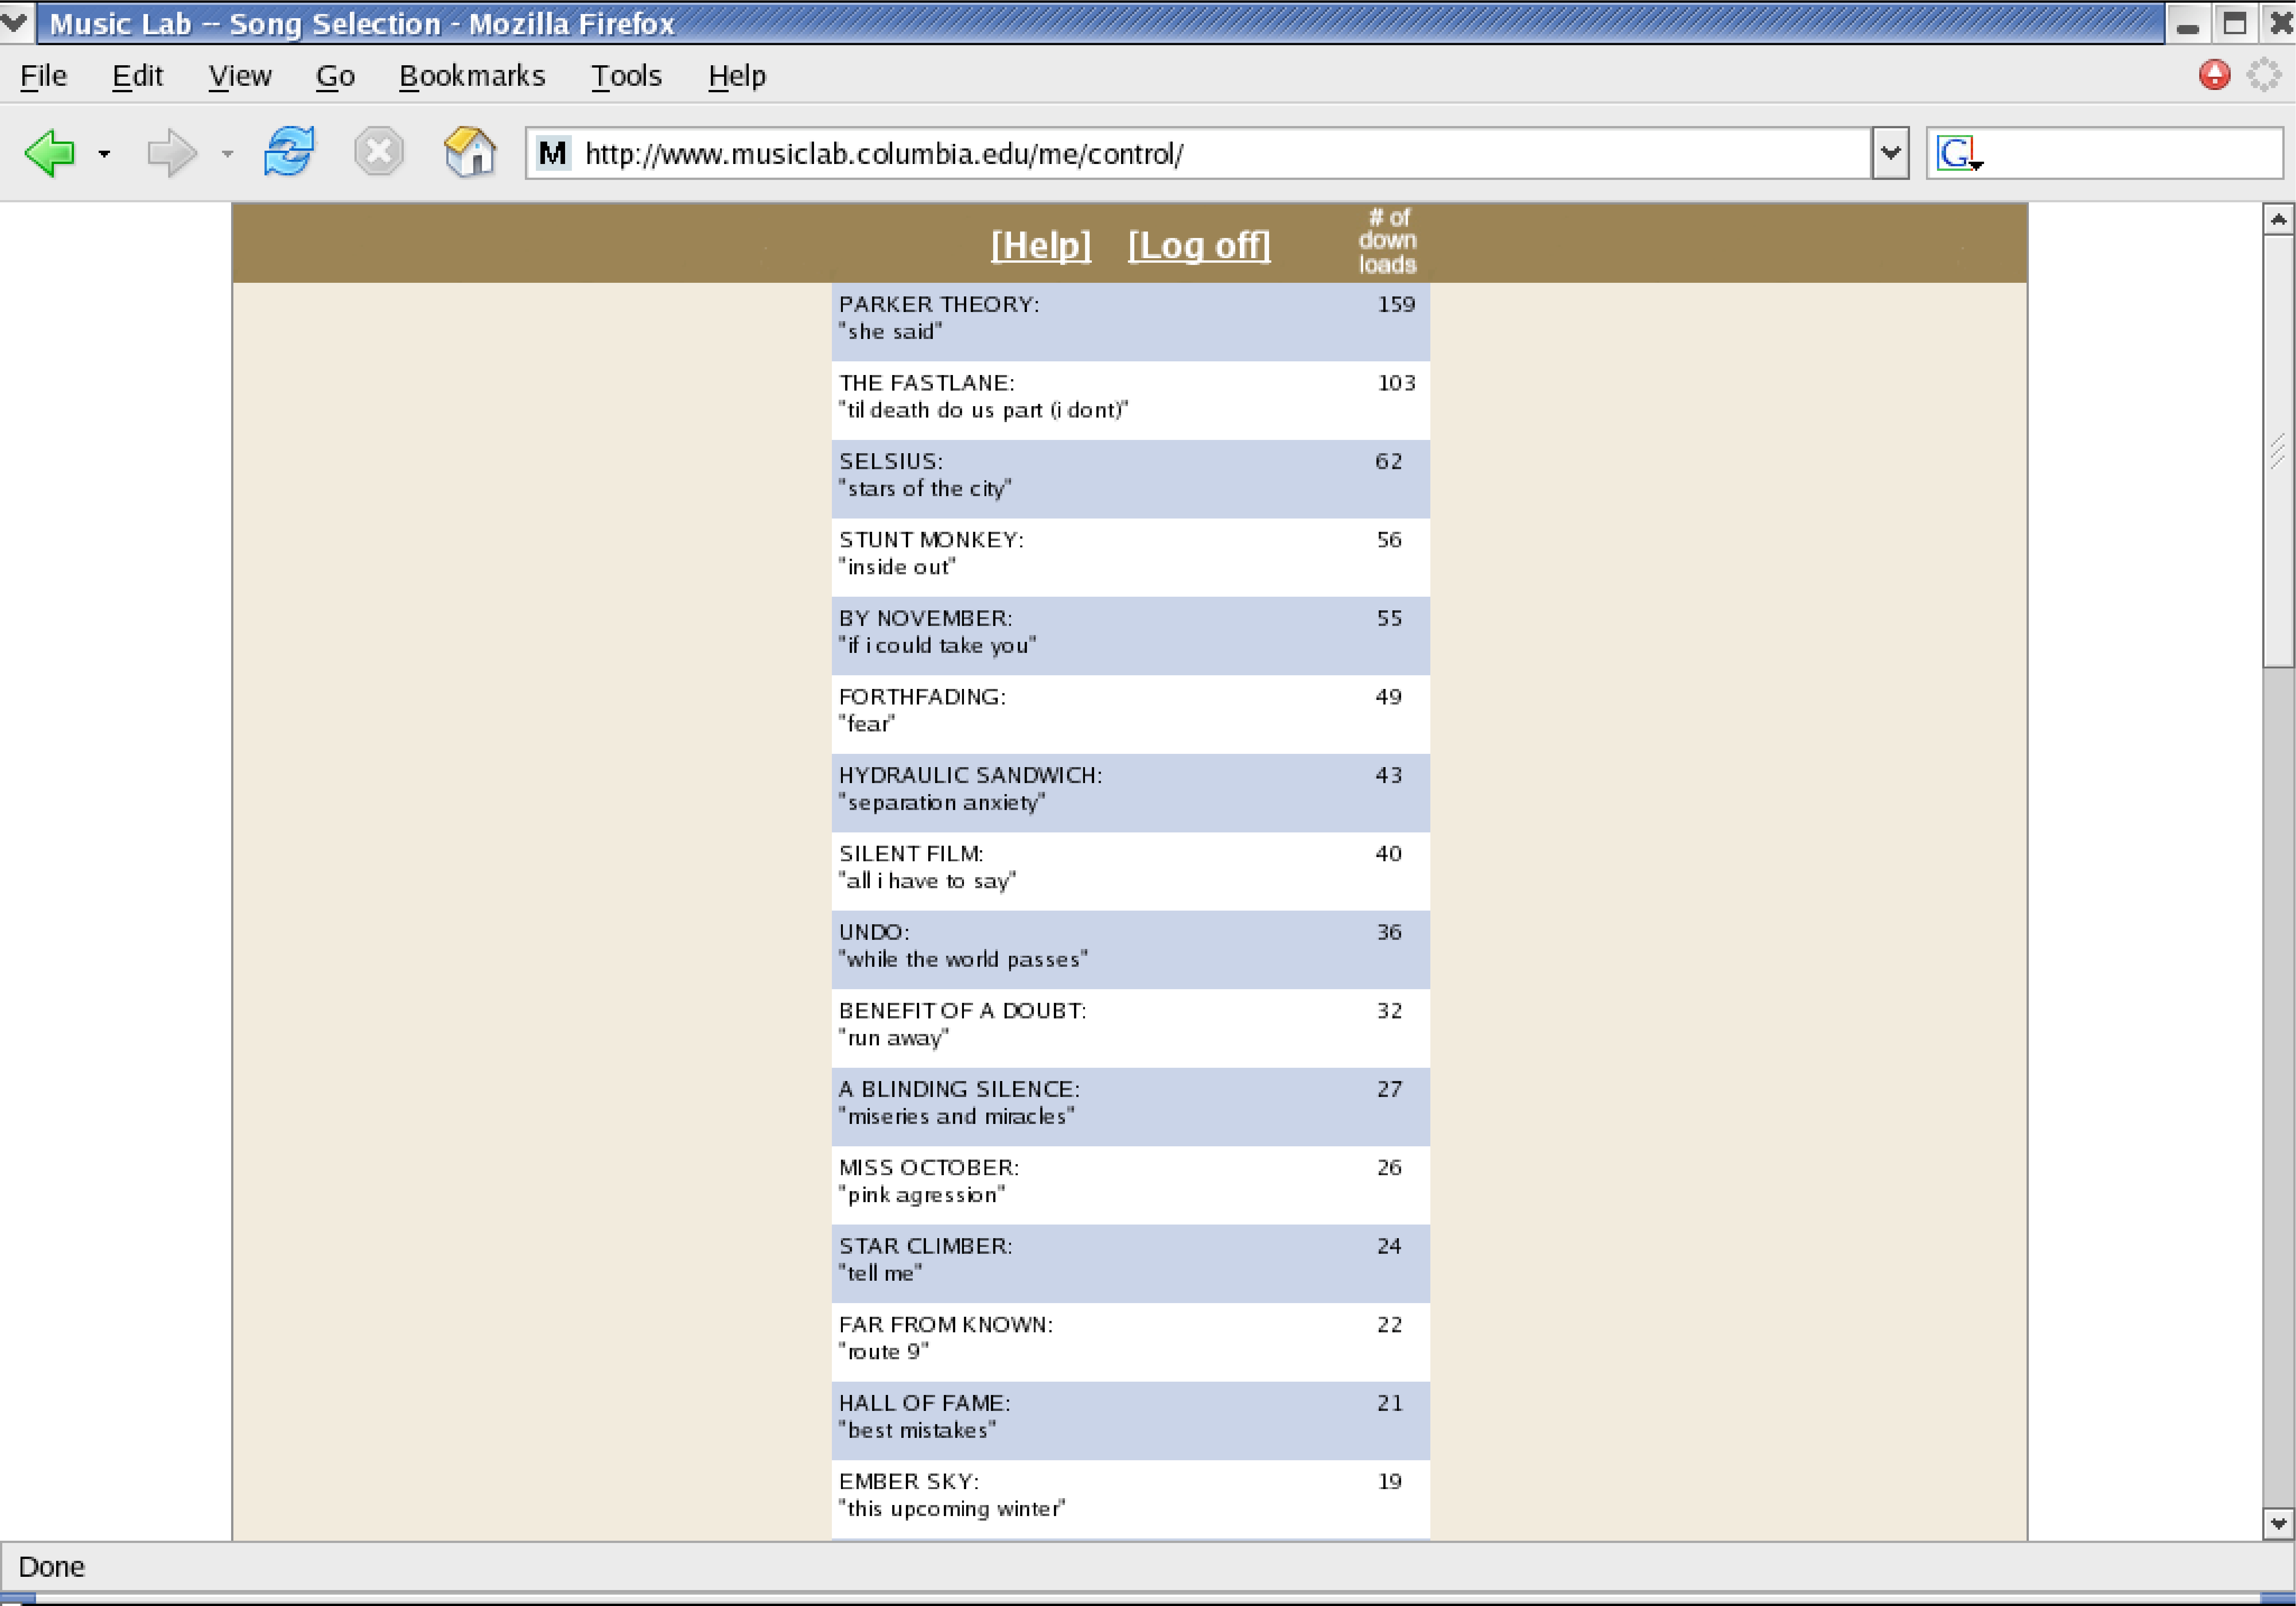
\includegraphics[width=0.45\textwidth]{figures/info-v2}}
\end{figure}

\end{frame}
%%%%%%%%%%%%%%%%%%%%%%%%%%%%%%
\begin{frame}

Two main measures
\begin{itemize}
\item Inequality
\item Unpredictability
\end{itemize}

\end{frame}
%%%%%%%%%%%%%%%%%%%%%%%%%%%%
\begin{frame}

\begin{figure}
  \centering
  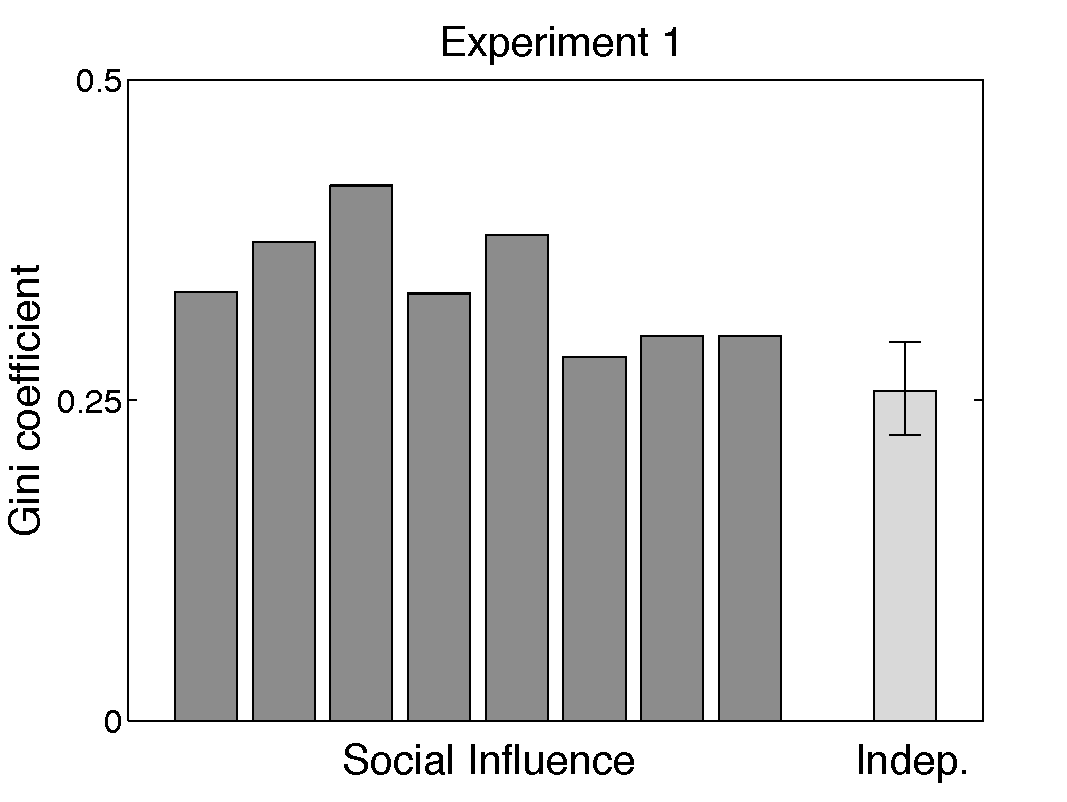
\includegraphics[width=0.7\textwidth]{figures/gini_v1_unordered_ci}
\end{figure}

\end{frame}
%%%%%%%%%%%%%%%%%%%%%%%%%%%%%%%%%%%%%%%%%%%%
\begin{frame}

\begin{figure}
  \centering
  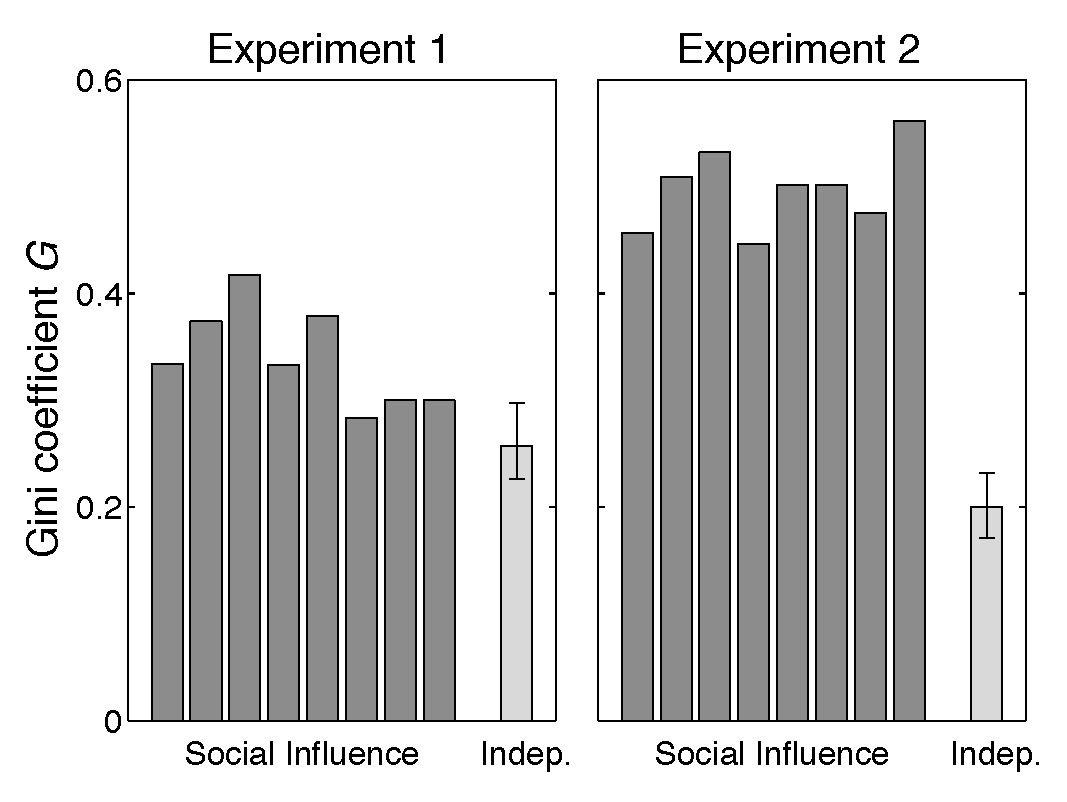
\includegraphics[width=3in]{figures/compare_gini_v1v2_unordered_ci}
\end{figure}

Median Gini coefficient increases from $0.34$ (France) to $0.50$ (Nigeria)
\end{frame}

%%%%%%%%%%%%%%%%%%%%%%%%%%%%%%%%%
\begin{frame}

\begin{figure}
  \centering
  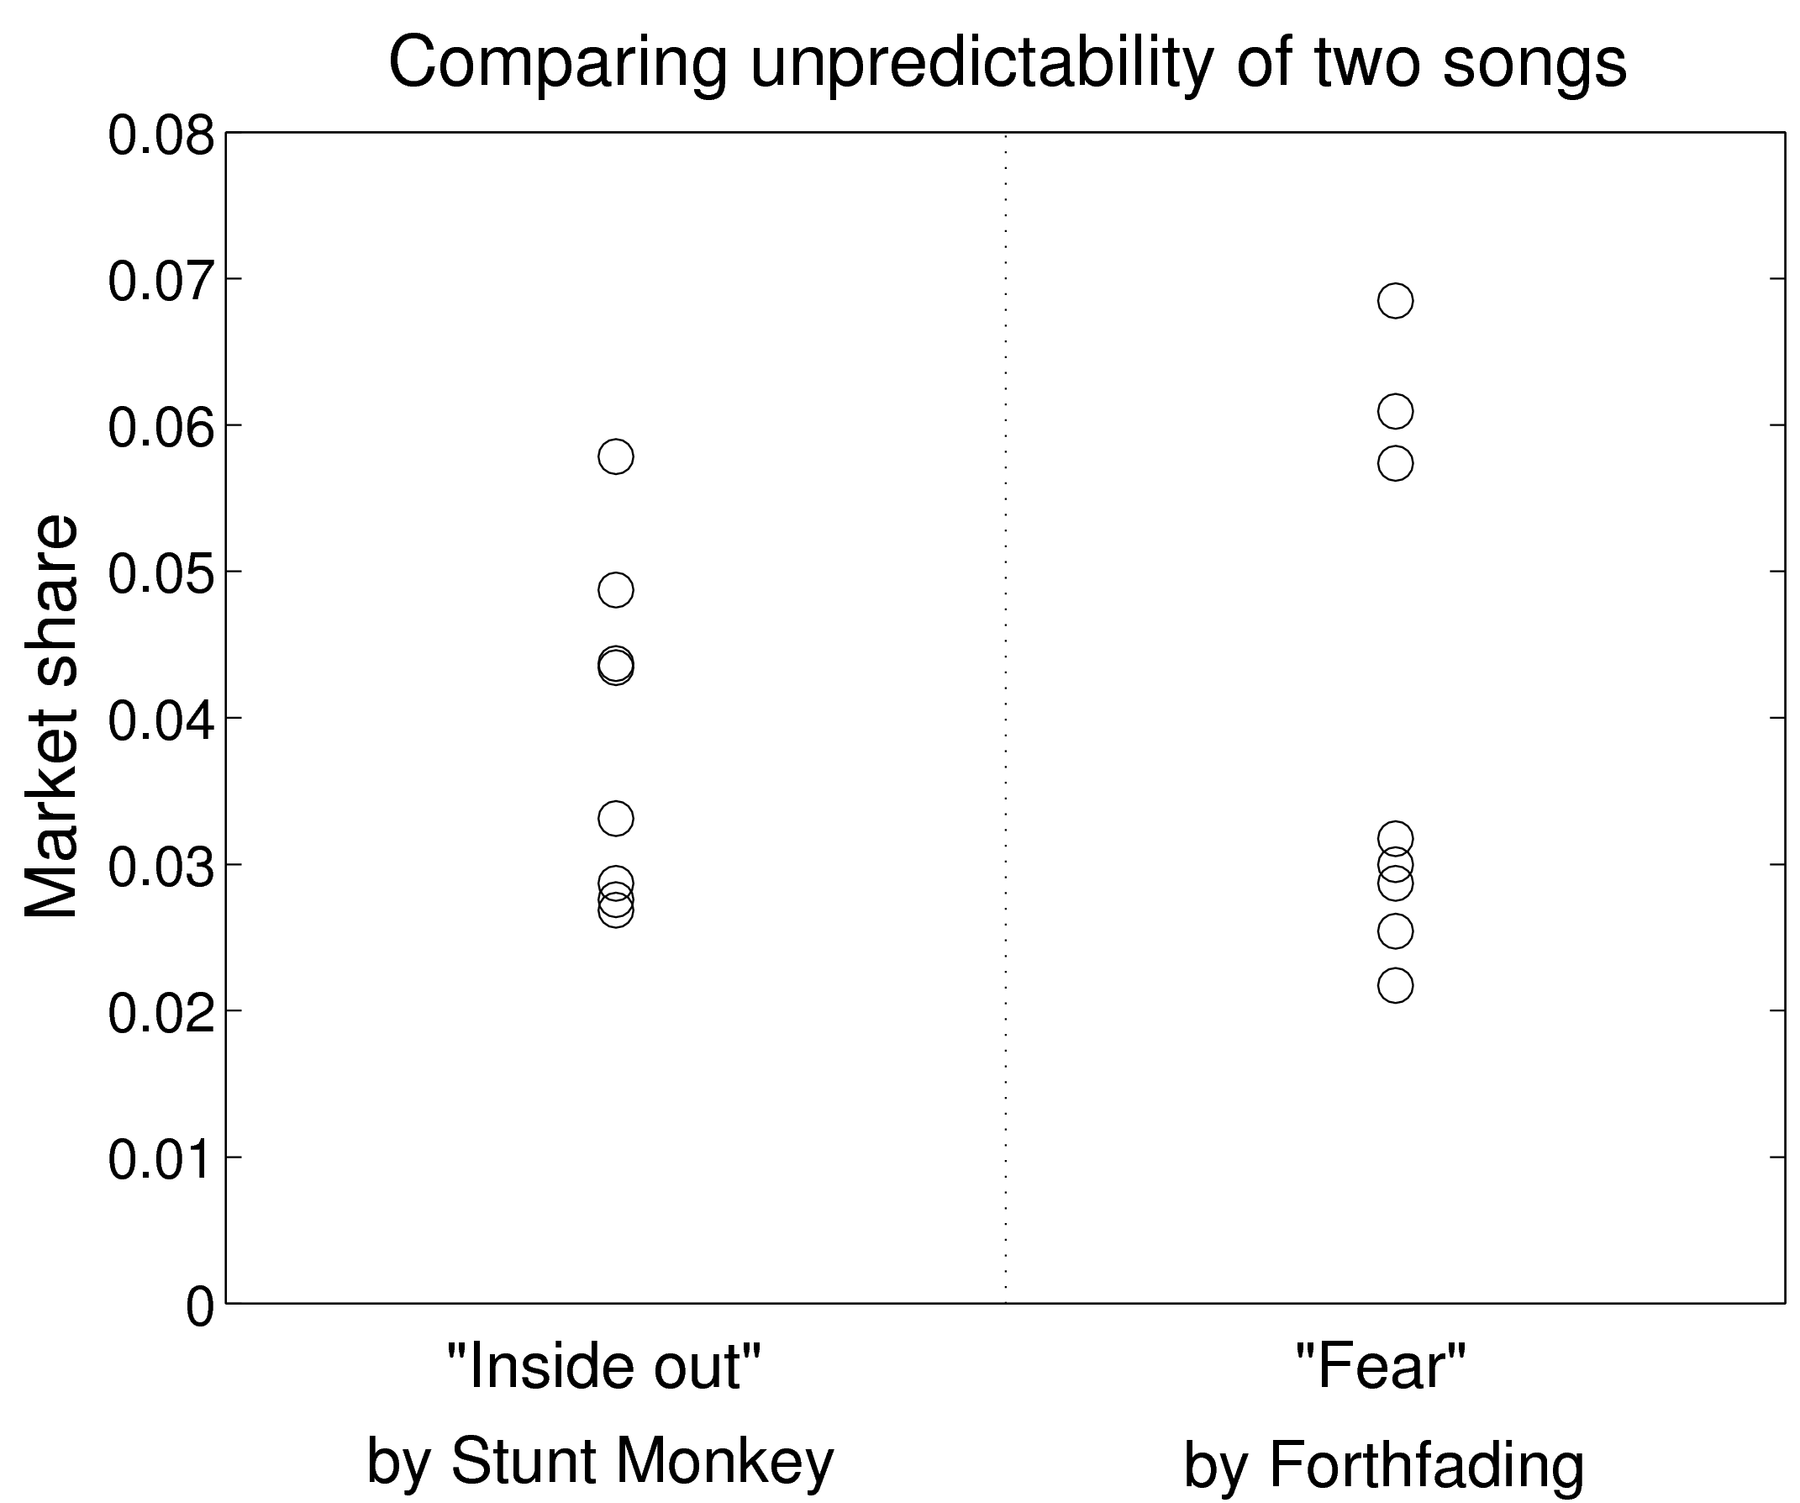
\includegraphics[width = 3in]{figures/arbitrary_example}
\end{figure}

$U$ = mean difference in market share across all pairs of realizations\\

\end{frame}
%%%%%%%%%%%%%%%%%%%%%%%%%%
\begin{frame}

\begin{figure}
  \centering
  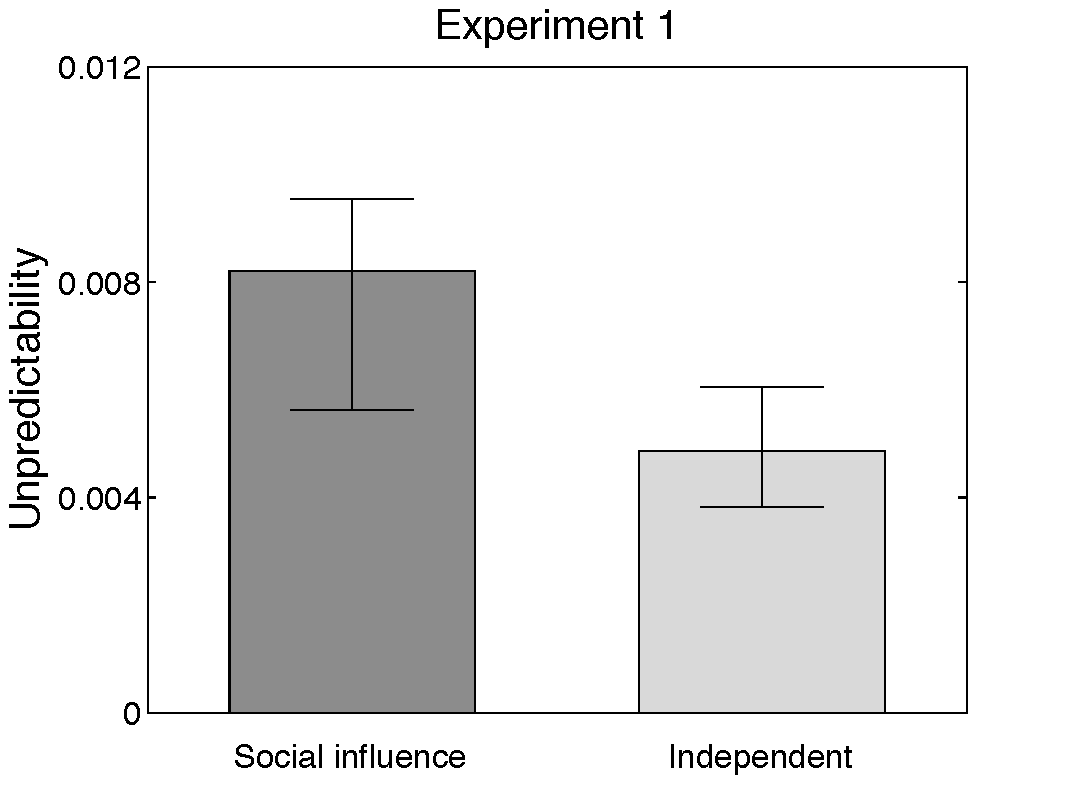
\includegraphics[width = 3.5in]{figures/unpredictability_v1}
\end{figure}

\end{frame}
%%%%%%%%%%%%%%%%%%%%%%%%%%%%
\begin{frame}

\begin{figure}
  \centering
  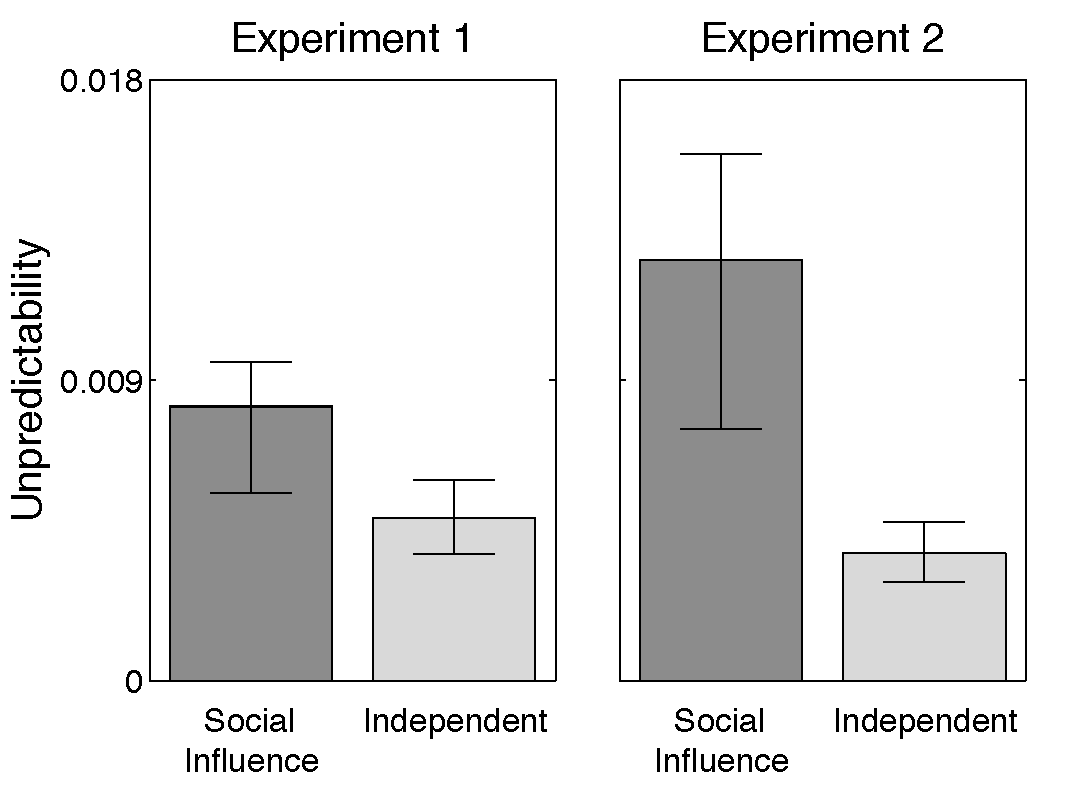
\includegraphics[width=3in]{figures/compare_unpred_v1v2}
\end{figure}

Unpredictability increases by about 50\%
\end{frame}
%%%%%%%%%%%%%%%%%%%%%%%%%%%%%%%%%
\begin{frame}

What is the relationship between ``quality'' and success?  Or expressed in terms of Martin et al. (2016) what is the relationship between ``skill'' and success?

\end{frame}
%%%%%%%%%%%%%%%%%%%%%%%%%%%%%%%%%%
\begin{frame}

\begin{center}
  \only<1>{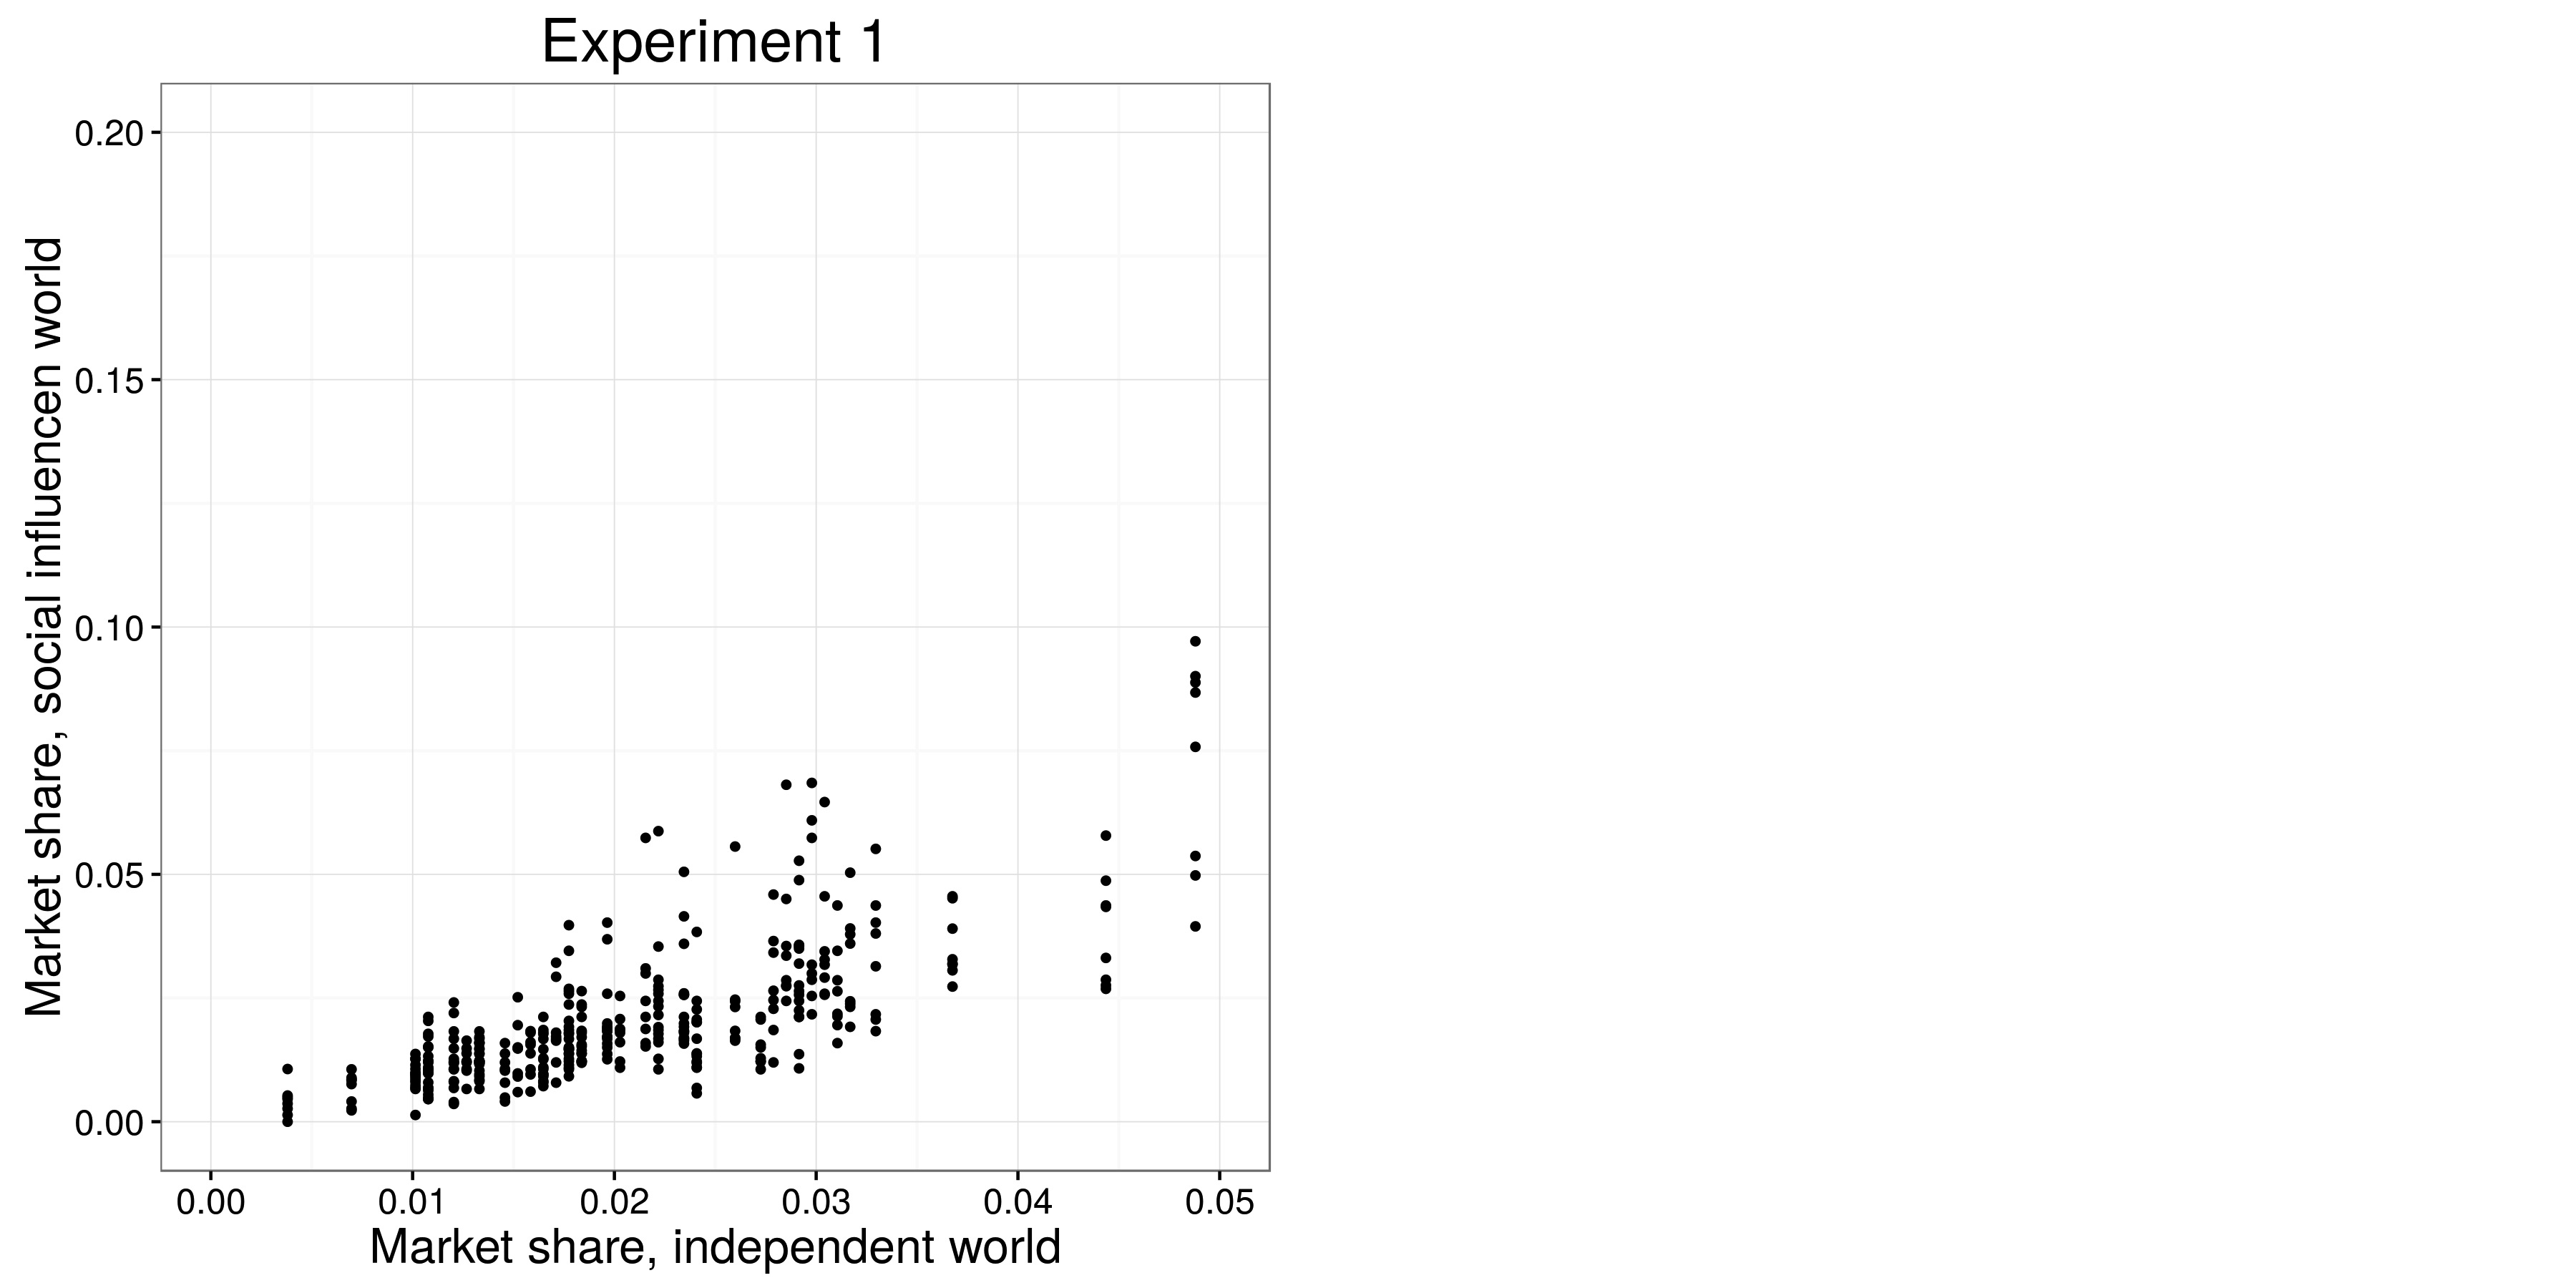
\includegraphics[width=0.9\textwidth]{figures/bitbybit4-23_salganik_experimental_2006_fig3a}}%
  \only<2>{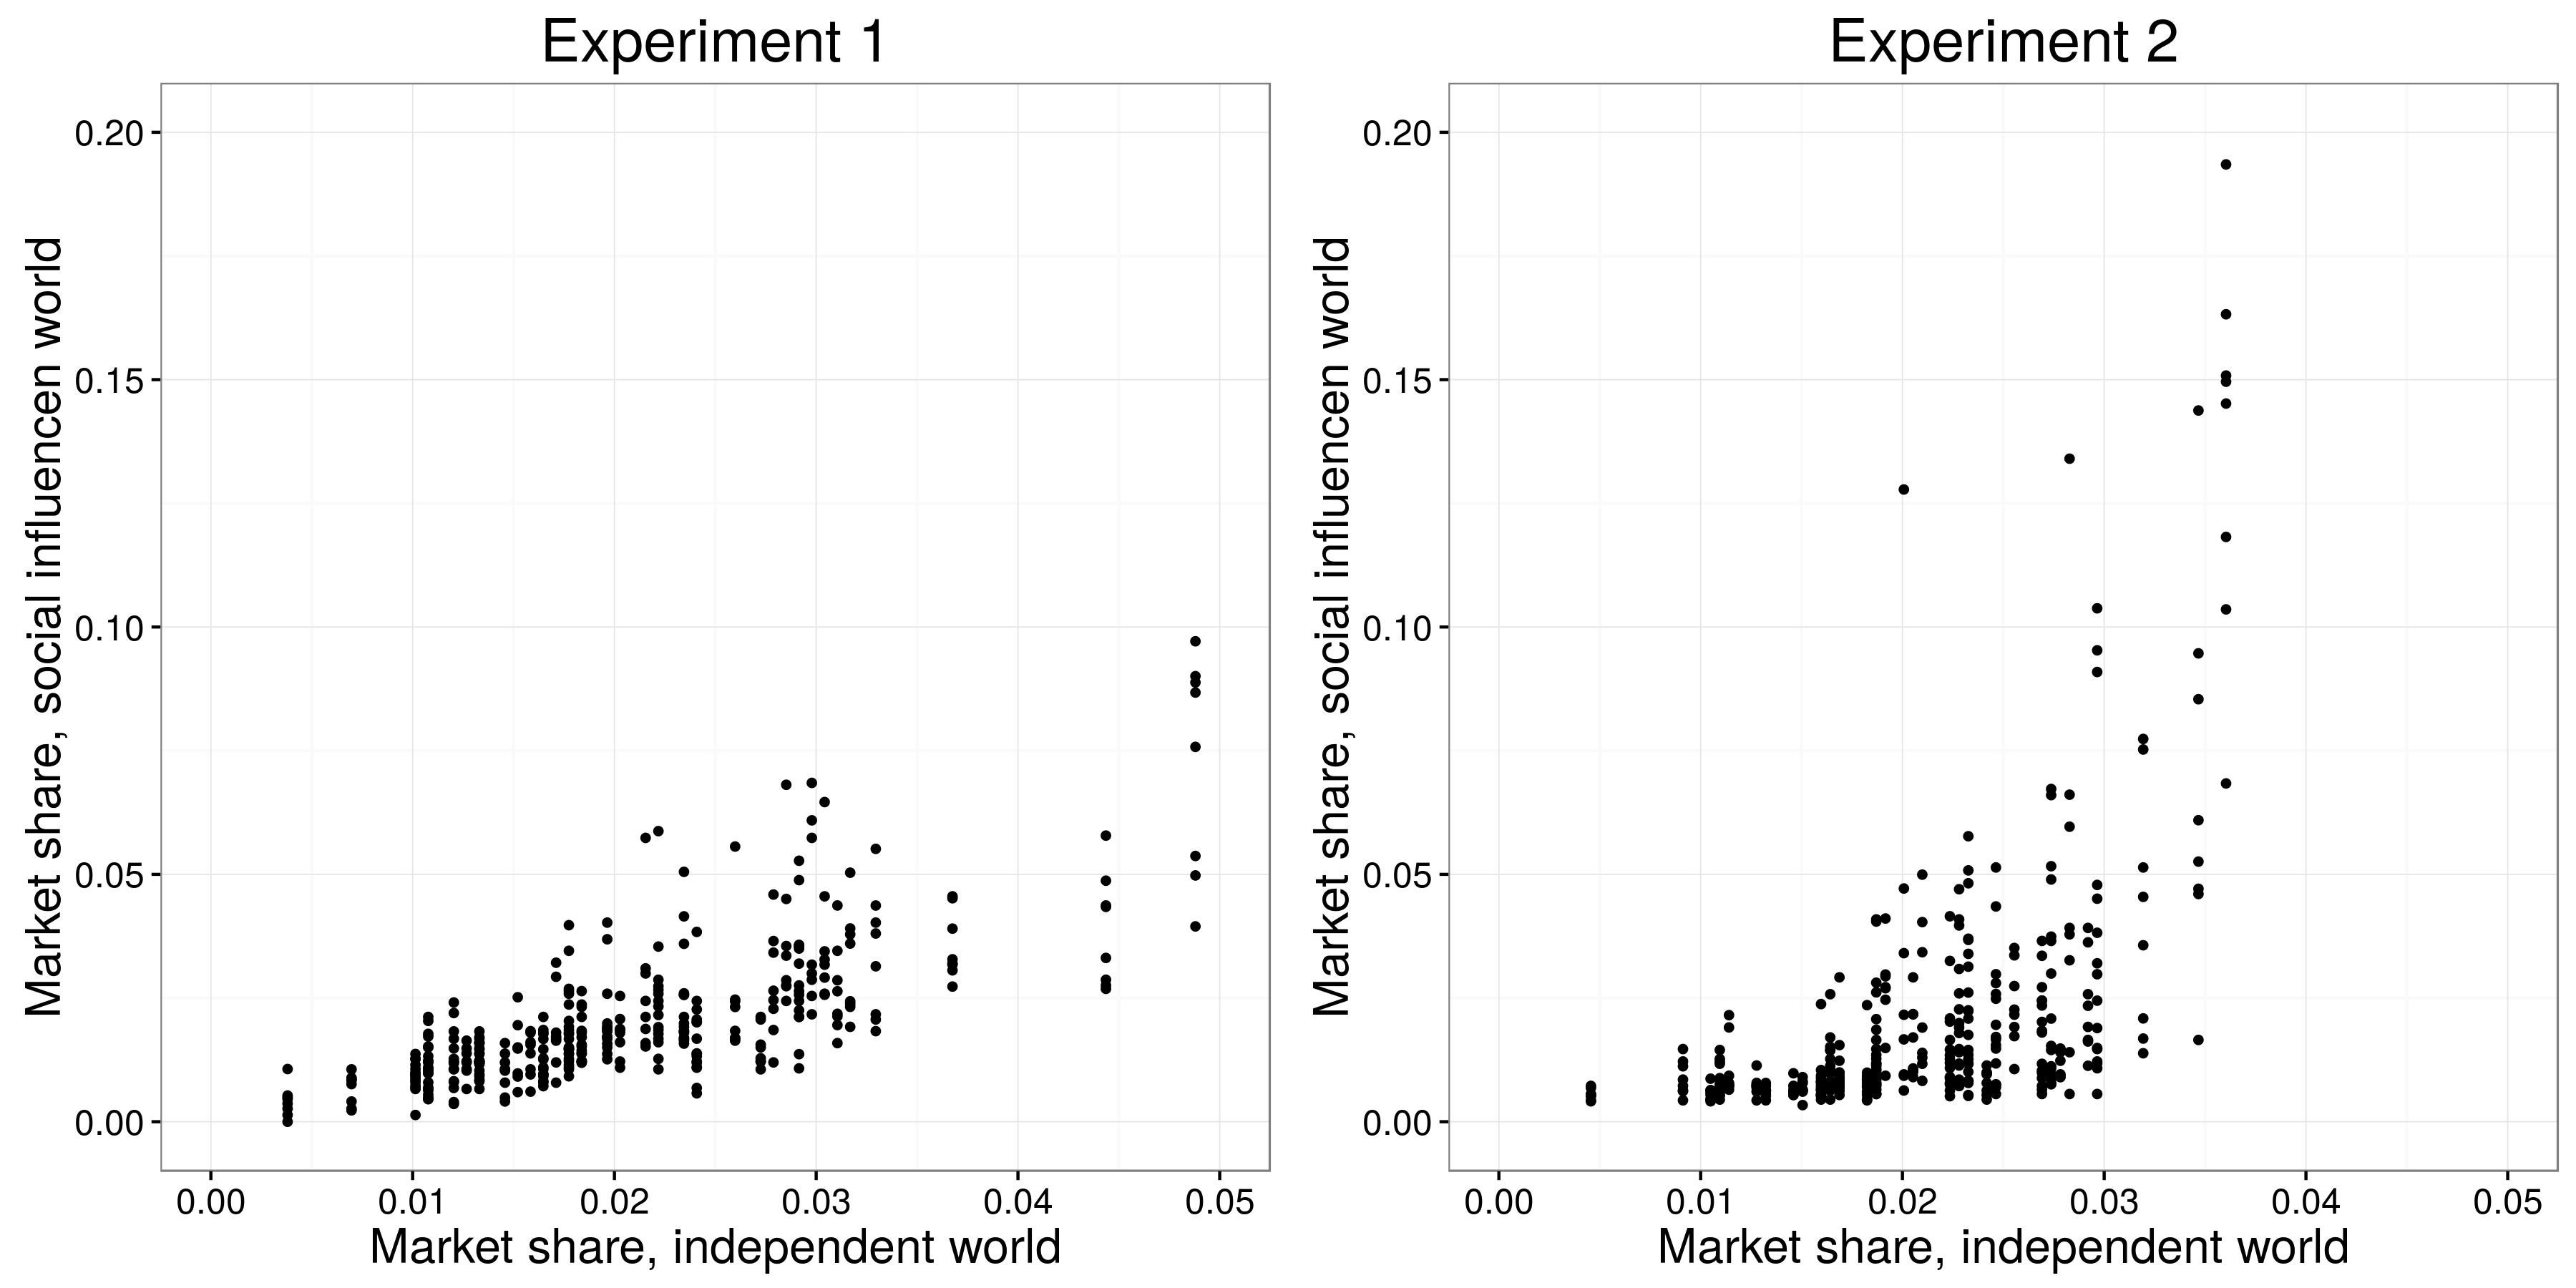
\includegraphics[width=0.9\textwidth]{figures/bitbybit4-23_salganik_experimental_2006_fig3ac}}%
\end{center}
 
\end{frame}
%%%%%%%%%%%%%%%%%%%%%%%%%%%%%%%%%%
\begin{frame}

\begin{center}
\LARGE{Behind the MusicLab}
\end{center}

\end{frame}
%%%%%%%%%%%%%%%%%%%%%%%%%%%%
\begin{frame}

Two main measures
\begin{itemize}
\item Inequality
\item Unpredictability
\end{itemize}

\end{frame}
%%%%%%%%%%%%%%%%%%%%%%%%%%%%
\begin{frame}

\begin{center}
  
\includegraphics[height=0.9\textheight]{figures/coulter_measuring_1989_cover.jpg}
\end{center}

\end{frame}
%%%%%%%%%%%%%%%%%%%%%%%%%%%%
\begin{frame}

\begin{center}
\only<1>{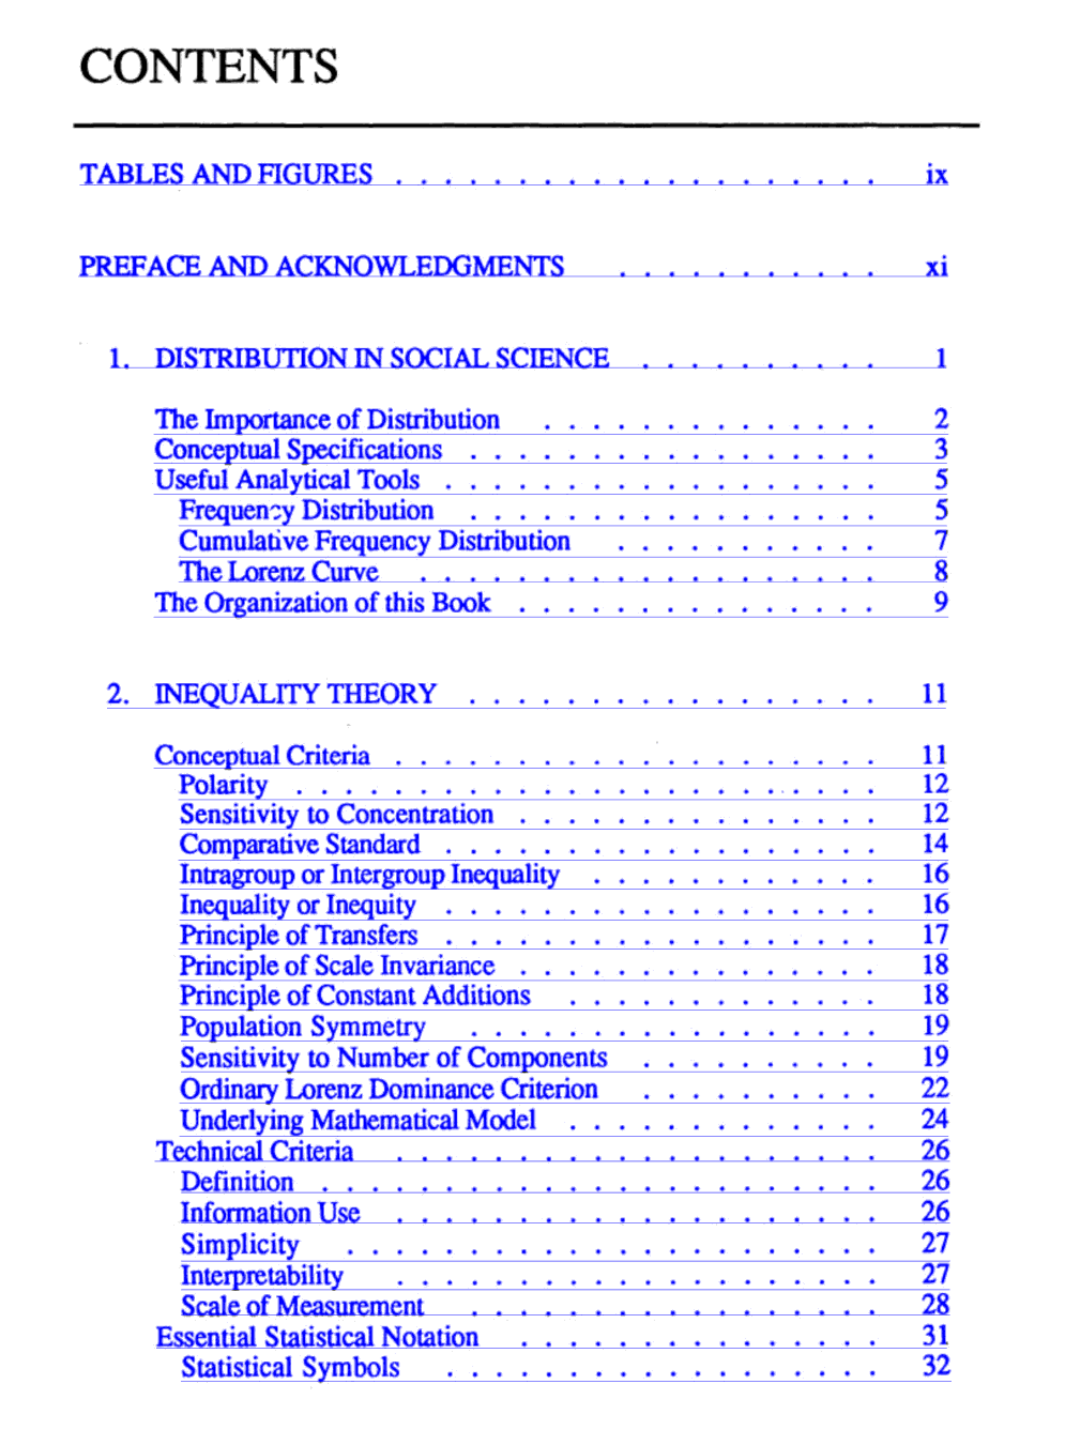
\includegraphics[height=0.9\textheight]{figures/coulter_measuring_1989_tc1}}%
\only<2>{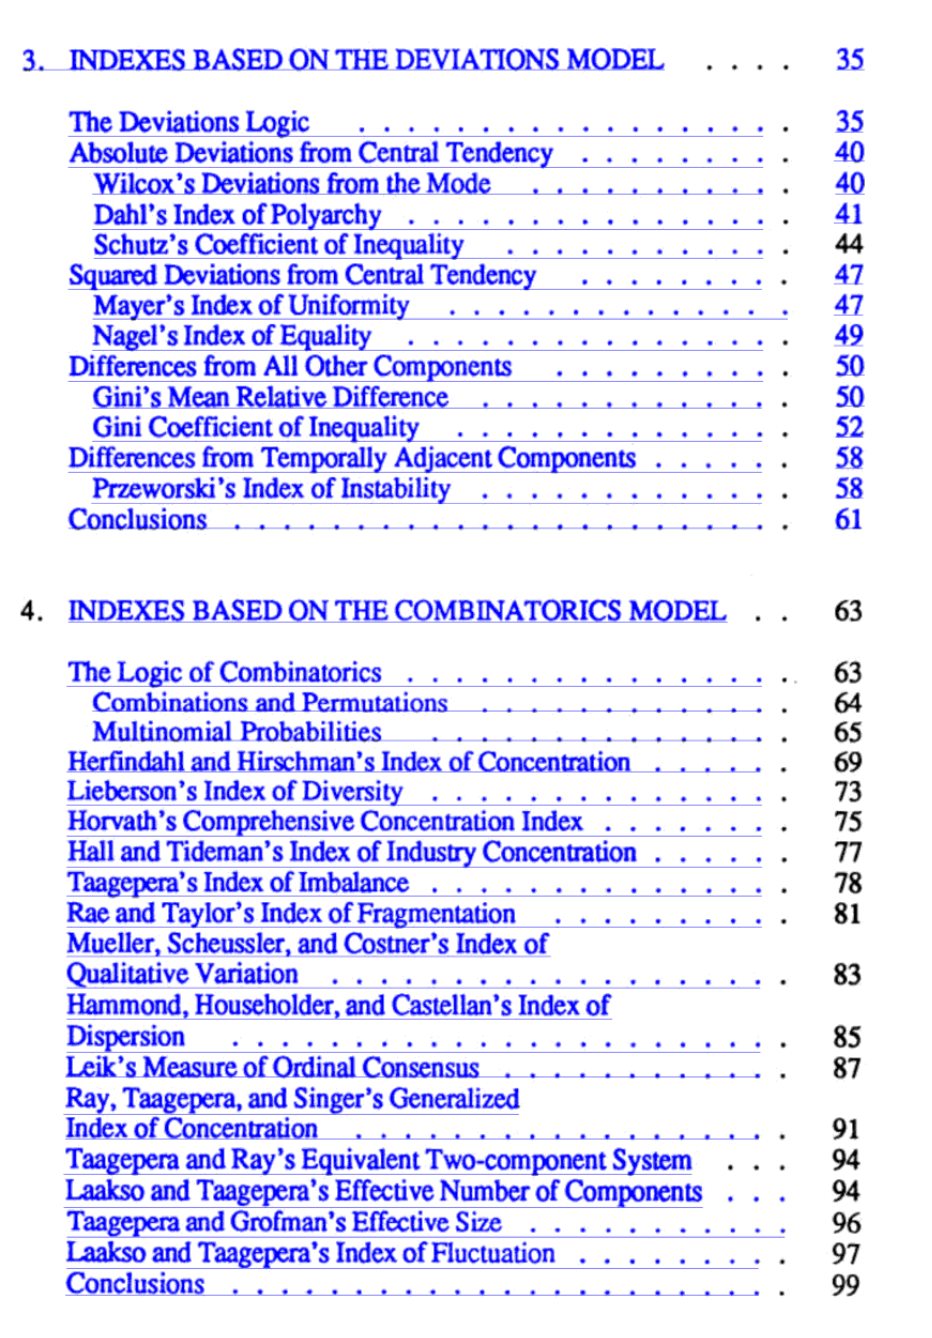
\includegraphics[height=0.9\textheight]{figures/coulter_measuring_1989_tc2}}%
\end{center}

\end{frame}
%%%%%%%%%%%%%%%%%%%%%%%%%%%%
\begin{frame}

\begin{center}
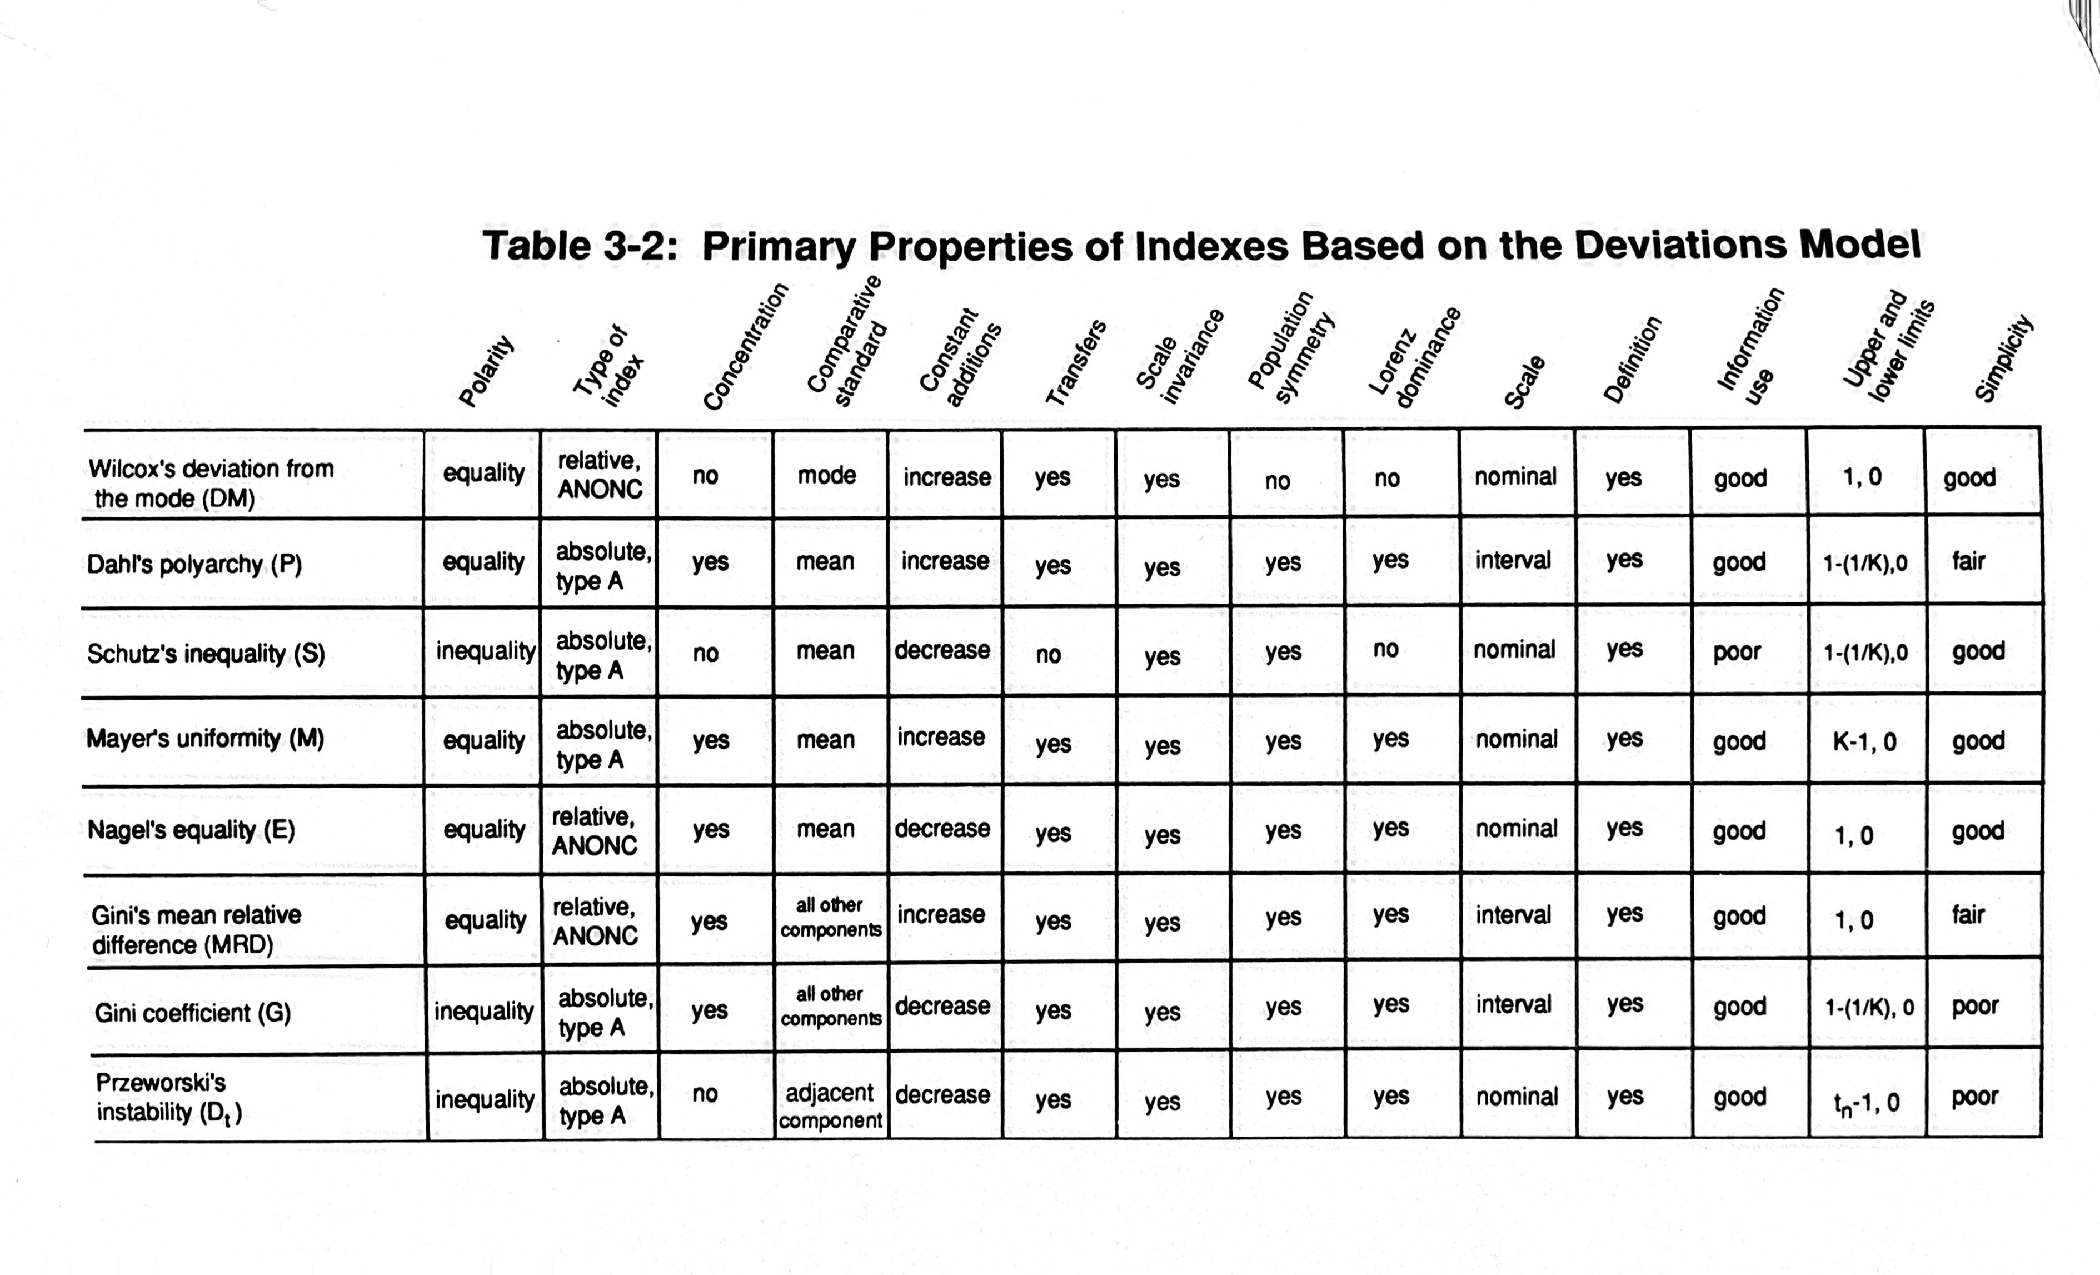
\includegraphics[width=0.9\textwidth]{figures/coulter_measuring_1989_tab3_2}
\end{center}

\end{frame}
%%%%%%%%%%%%%%%%%%%%%%%%%%%%
\begin{frame}

\begin{figure}
  \centering
  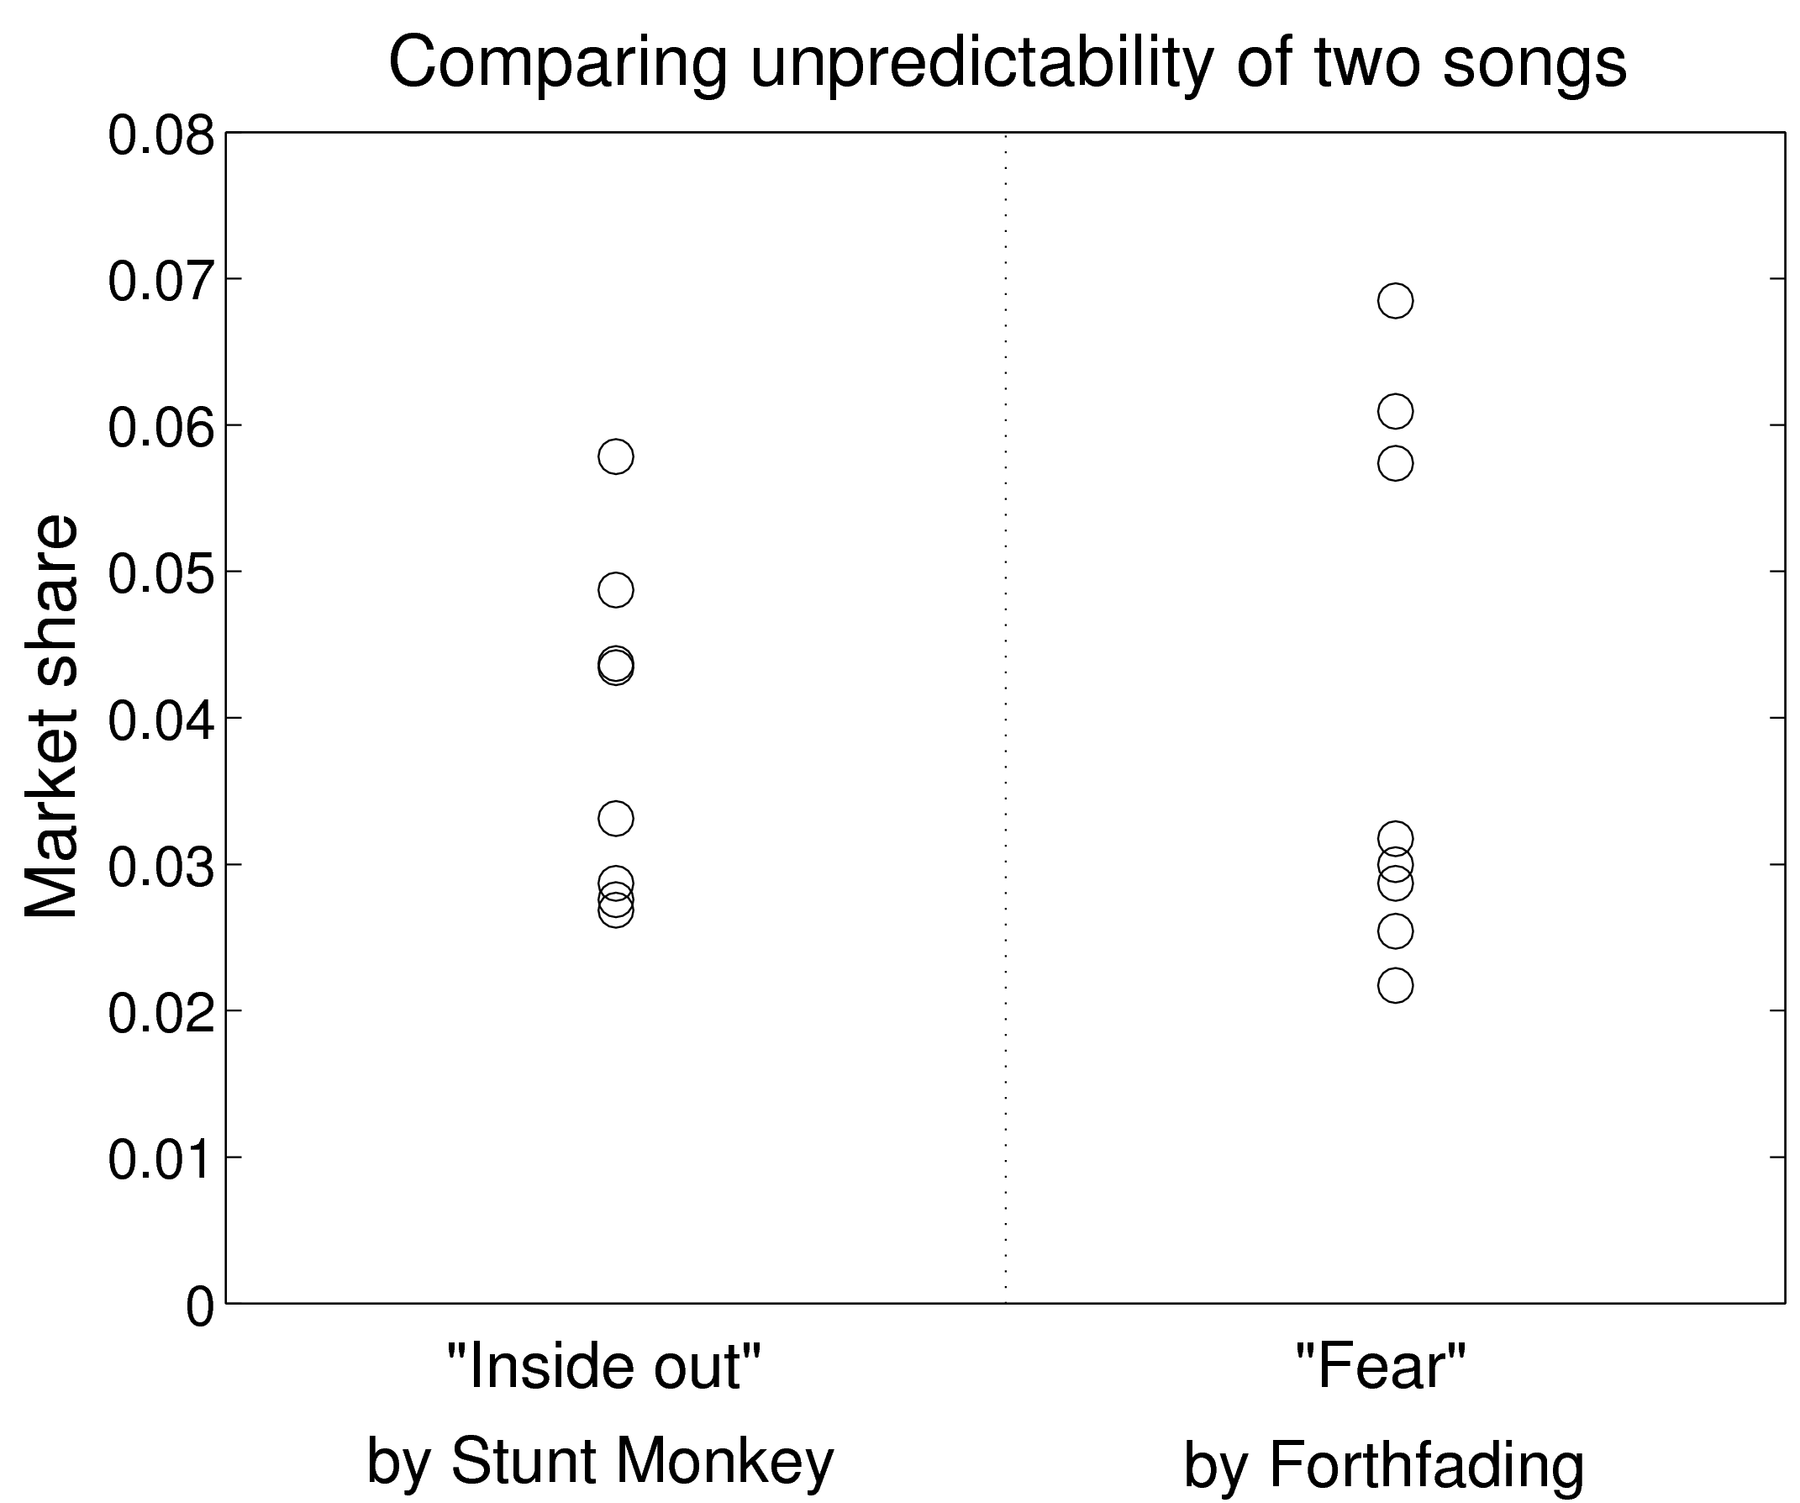
\includegraphics[width = 3in]{figures/arbitrary_example}
\end{figure}

$U$ = mean difference in market share across all pairs of realizations

\end{frame}
%%%%%%%%%%%%%%%%%%%%%%%%%%
\begin{frame}

\begin{center}
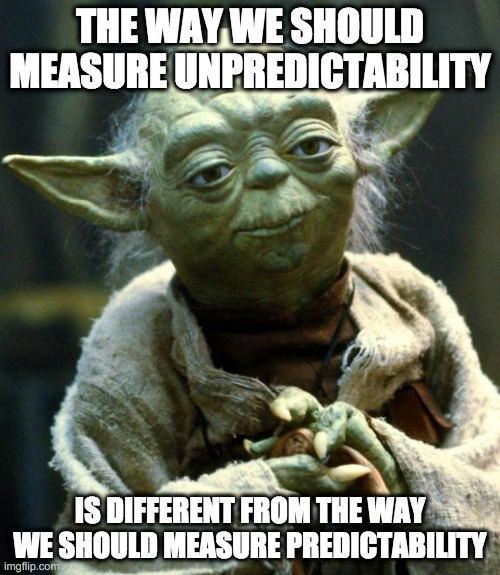
\includegraphics[height=0.9\textheight]{figures/the_way_we_should_unpredictability}
\end{center}

\end{frame}
%%%%%%%%%%%%%%%%%%%%%%%%%%%
\begin{frame}

How did we come to study unpredictability?

\end{frame}
%%%%%%%%%%%%%%%%%%%%%%%%%%%%
\begin{frame}

\begin{center}
  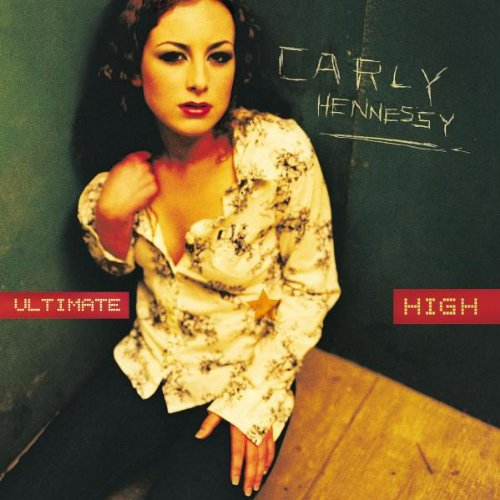
\includegraphics[width = 0.5\textwidth]{figures/hennessy_ultimate_2006_cover}
\end{center}

\vfill

\url{https://www.youtube.com/watch?v=2wfhk46_tXE}

\end{frame}
%%%%%%%%%%%%%%%%%%%%%%%%%%%%
\begin{frame}

\begin{center}
  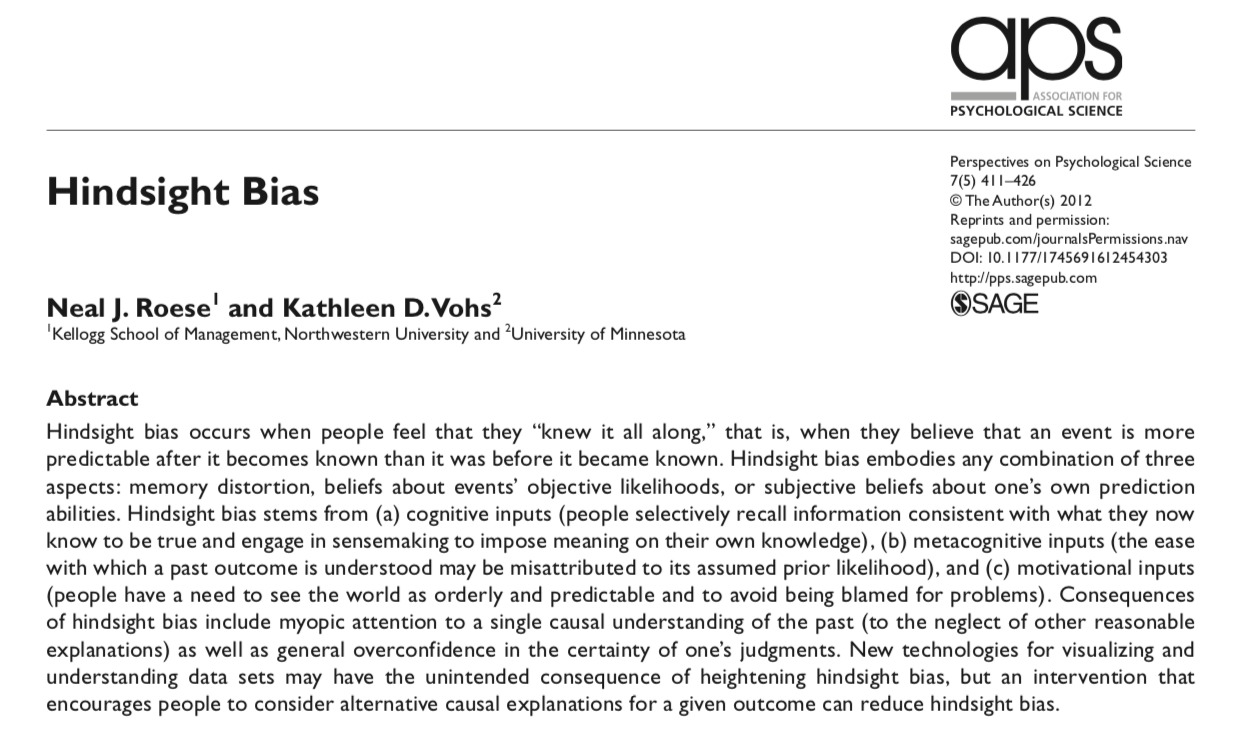
\includegraphics[width = 0.9\textwidth]{figures/roese_hindsight_2012_title_abstract}
\end{center}

\end{frame}
%%%%%%%%%%%%%%%%%%%%%%%%%%%%
\begin{frame}

\begin{center}
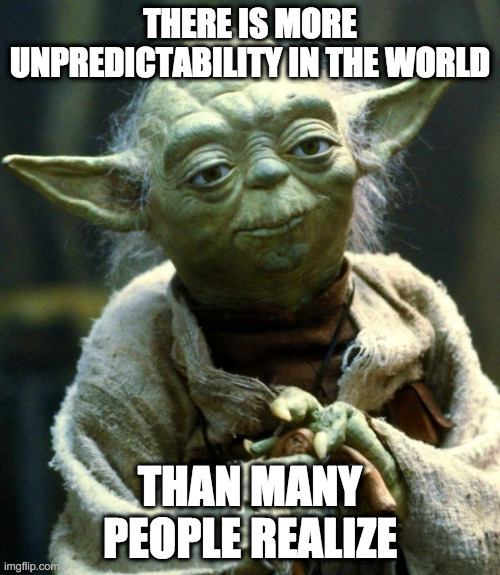
\includegraphics[height=0.9\textheight]{figures/there_is_more}
\end{center}

\end{frame}
%%%%%%%%%%%%%%%%%%%%%%%%%%%
\begin{frame}

\begin{center}
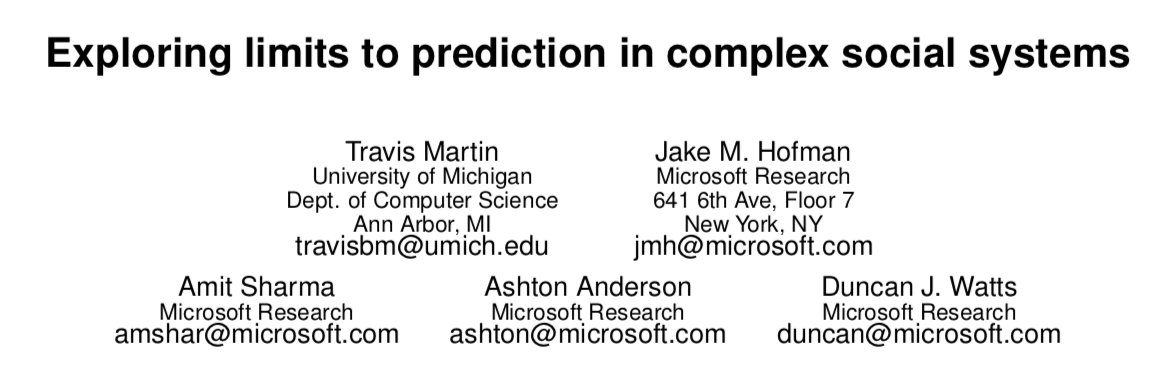
\includegraphics[width=0.9\textwidth]{figures/martin_exploring_2016_title}
\end{center}

\end{frame}
%%%%%%%%%%%%%%%%%%%%%%%%%%%
\begin{frame}

\begin{center}
\only<1>{
\includegraphics[width = 0.7\textwidth]{figures/arvind_tweet_nocount}}%
\only<2>{
\includegraphics[width = 0.7\textwidth]{figures/arvind_tweet_wcount}}%
\end{center}

\end{frame}
%%%%%%%%%%%%%%%%%%%%%%%%%%
\begin{frame}

\begin{center}
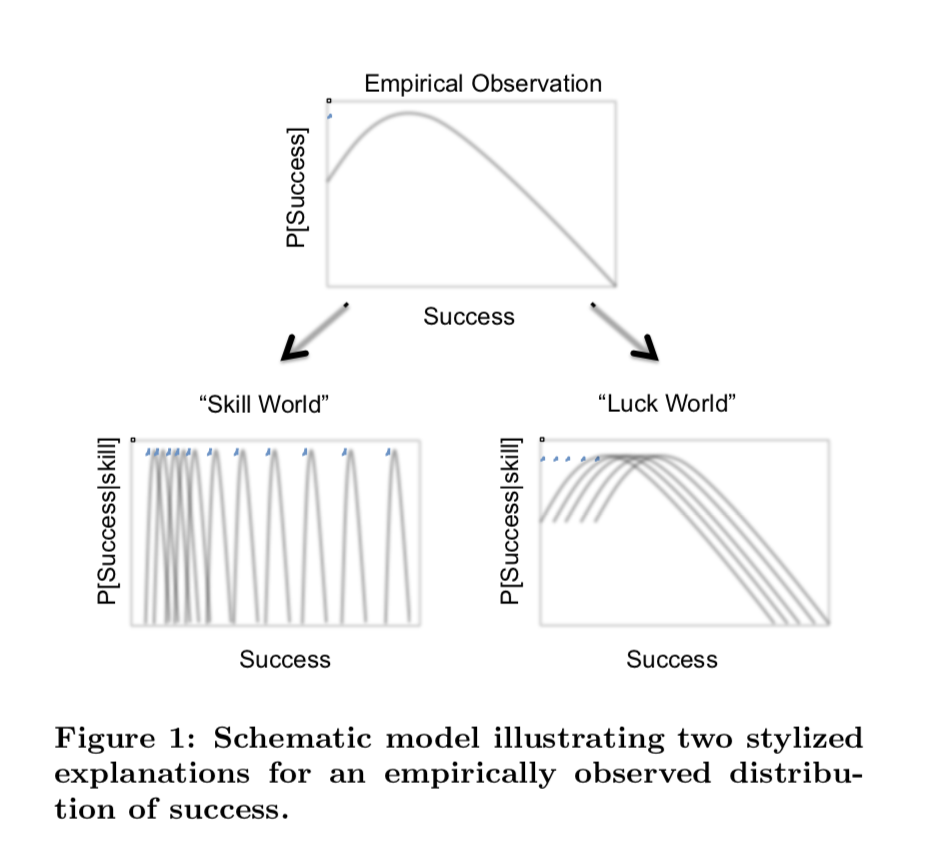
\includegraphics[width=0.7\textwidth]{figures/martin_exploring_2016_fig1}
\end{center}

\end{frame}
%%%%%%%%%%%%%%%%%%%%%%%%%%%
\begin{frame}

$s  = f(q) + \epsilon$

\end{frame}
%%%%%%%%%%%%%%%%%%%%%%%%%%%
\begin{frame}

\begin{center}
\only<1>{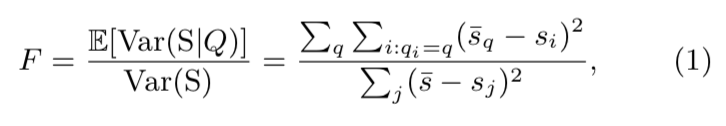
\includegraphics[width=0.9\textwidth]{figures/martin_exploring_2016_eq1}}%
\only<2>{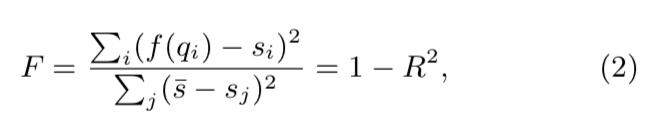
\includegraphics[width=0.9\textwidth]{figures/martin_exploring_2016_eq2}}%
\end{center}

\end{frame}
%%%%%%%%%%%%%%%%%%%%%%%%%%%
\begin{frame}

\begin{center}
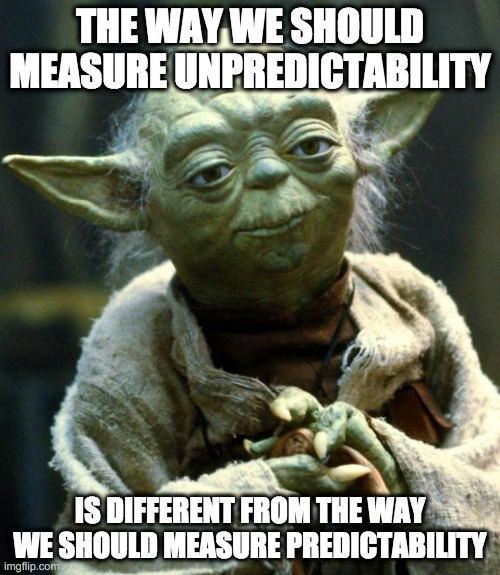
\includegraphics[height=0.9\textheight]{figures/the_way_we_should_unpredictability}
\end{center}

\end{frame}
%%%%%%%%%%%%%%%%%%%%%%%%%%%
\begin{frame}

\begin{center}
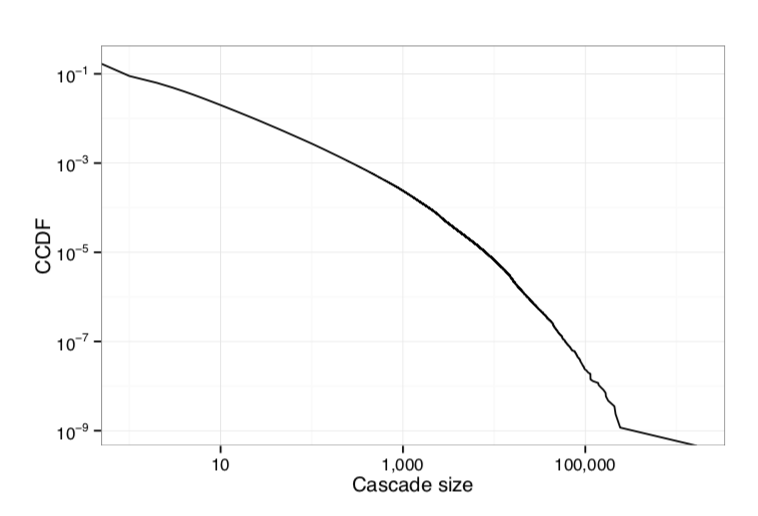
\includegraphics[width=0.7\textwidth]{figures/martin_exploring_2016_fig2b}
\end{center}

\vfill
I believe that it is in general hard to predict outcomes with more variation.  Is that true?
\end{frame}
%%%%%%%%%%%%%%%%%%%%%%%%%%%
\begin{frame}

\begin{center}
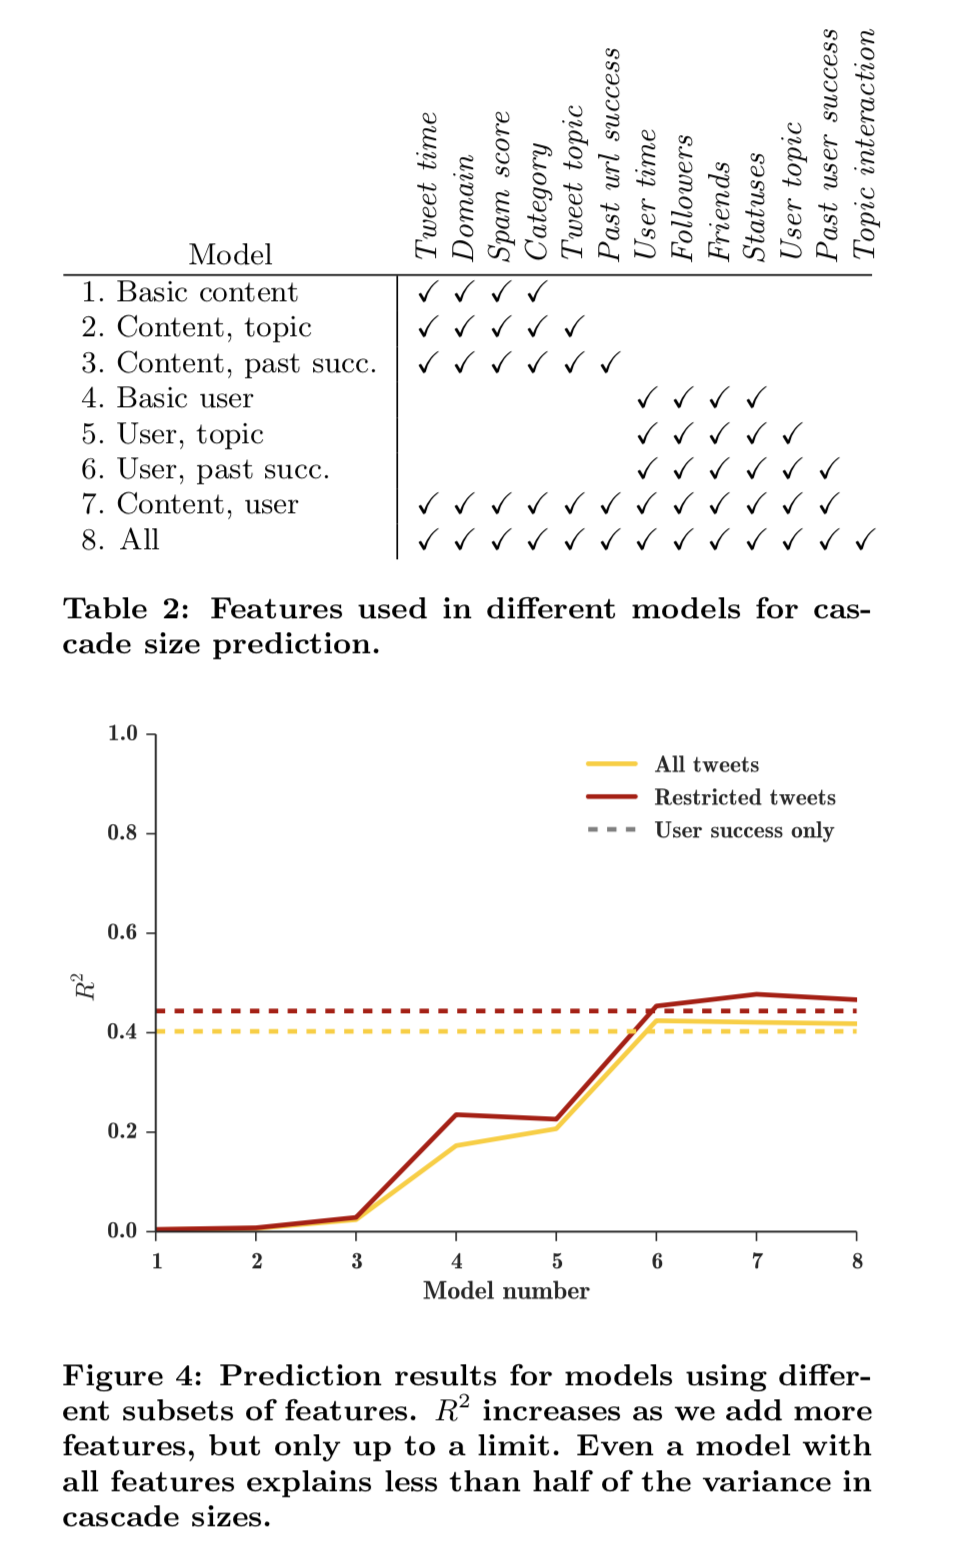
\includegraphics[height=0.8\textheight]{figures/martin_exploring_2016_tab2_fig4}
\end{center}

\pause
\vfill
What about my favorite feature? What about deep learning? What about . . . .

\end{frame}
%%%%%%%%%%%%%%%%%%%%%%%%%%%
\begin{frame}

They don't close the loop. It is very hard to get the simulation results and the empirical results to work together tightly.

\end{frame}
%%%%%%%%%%%%%%%%%%%%%%%%%%%%%%%%
\begin{frame}

\begin{center}
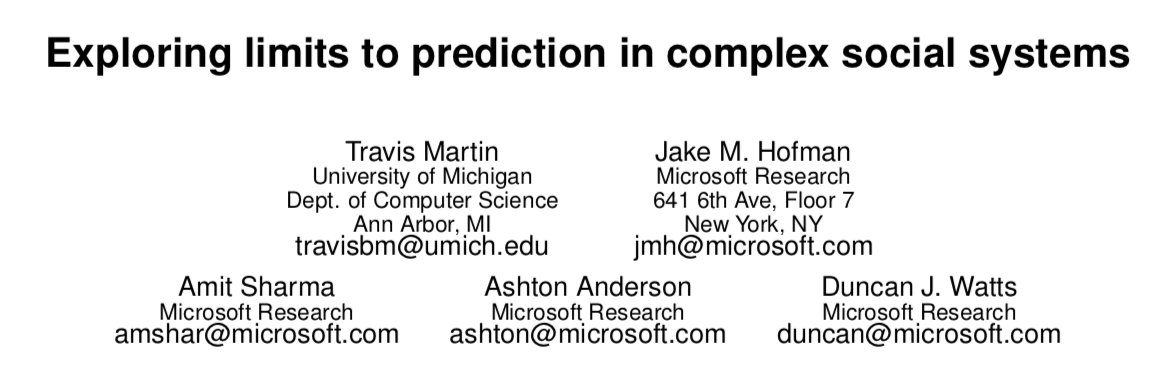
\includegraphics[width=0.9\textwidth]{figures/martin_exploring_2016_title}
\end{center}

\end{frame}
%%%%%%%%%%%%%%%%%%%%%%%%%%%
\begin{frame}

\begin{center}
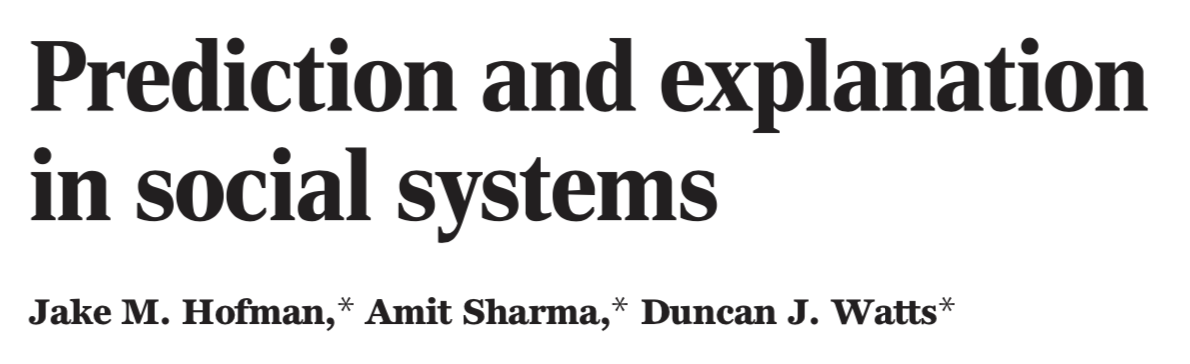
\includegraphics[width=0.9\textwidth]{figures/hofman_prediction_2017_title}
\end{center}

\end{frame}
%%%%%%%%%%%%%%%%%%%%%%%%%%%%%
\begin{frame}

\begin{center}
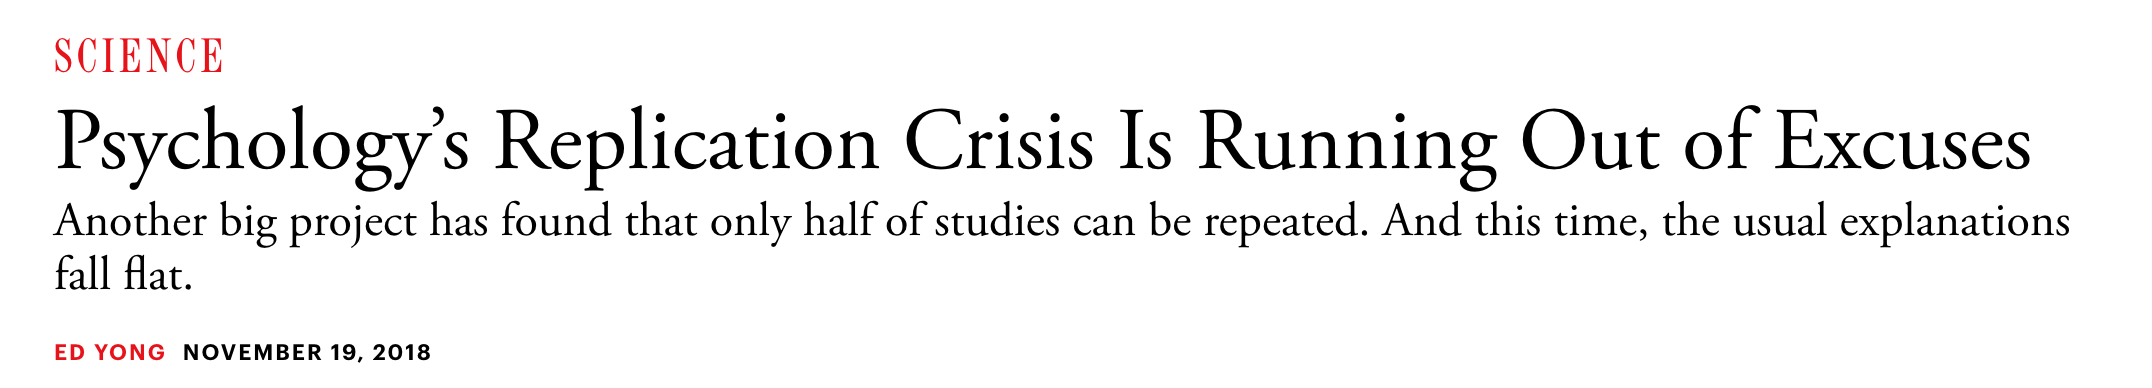
\includegraphics[width=0.9\textwidth]{figures/yong_psychologys_2018_title}
\end{center}

\vfill
\url{https://www.theatlantic.com/science/archive/2018/11/psychologys-replication-crisis-real/576223/}

\end{frame}
%%%%%%%%%%%%%%%%%%%%%%%%%%%%
\begin{frame}

\begin{center}
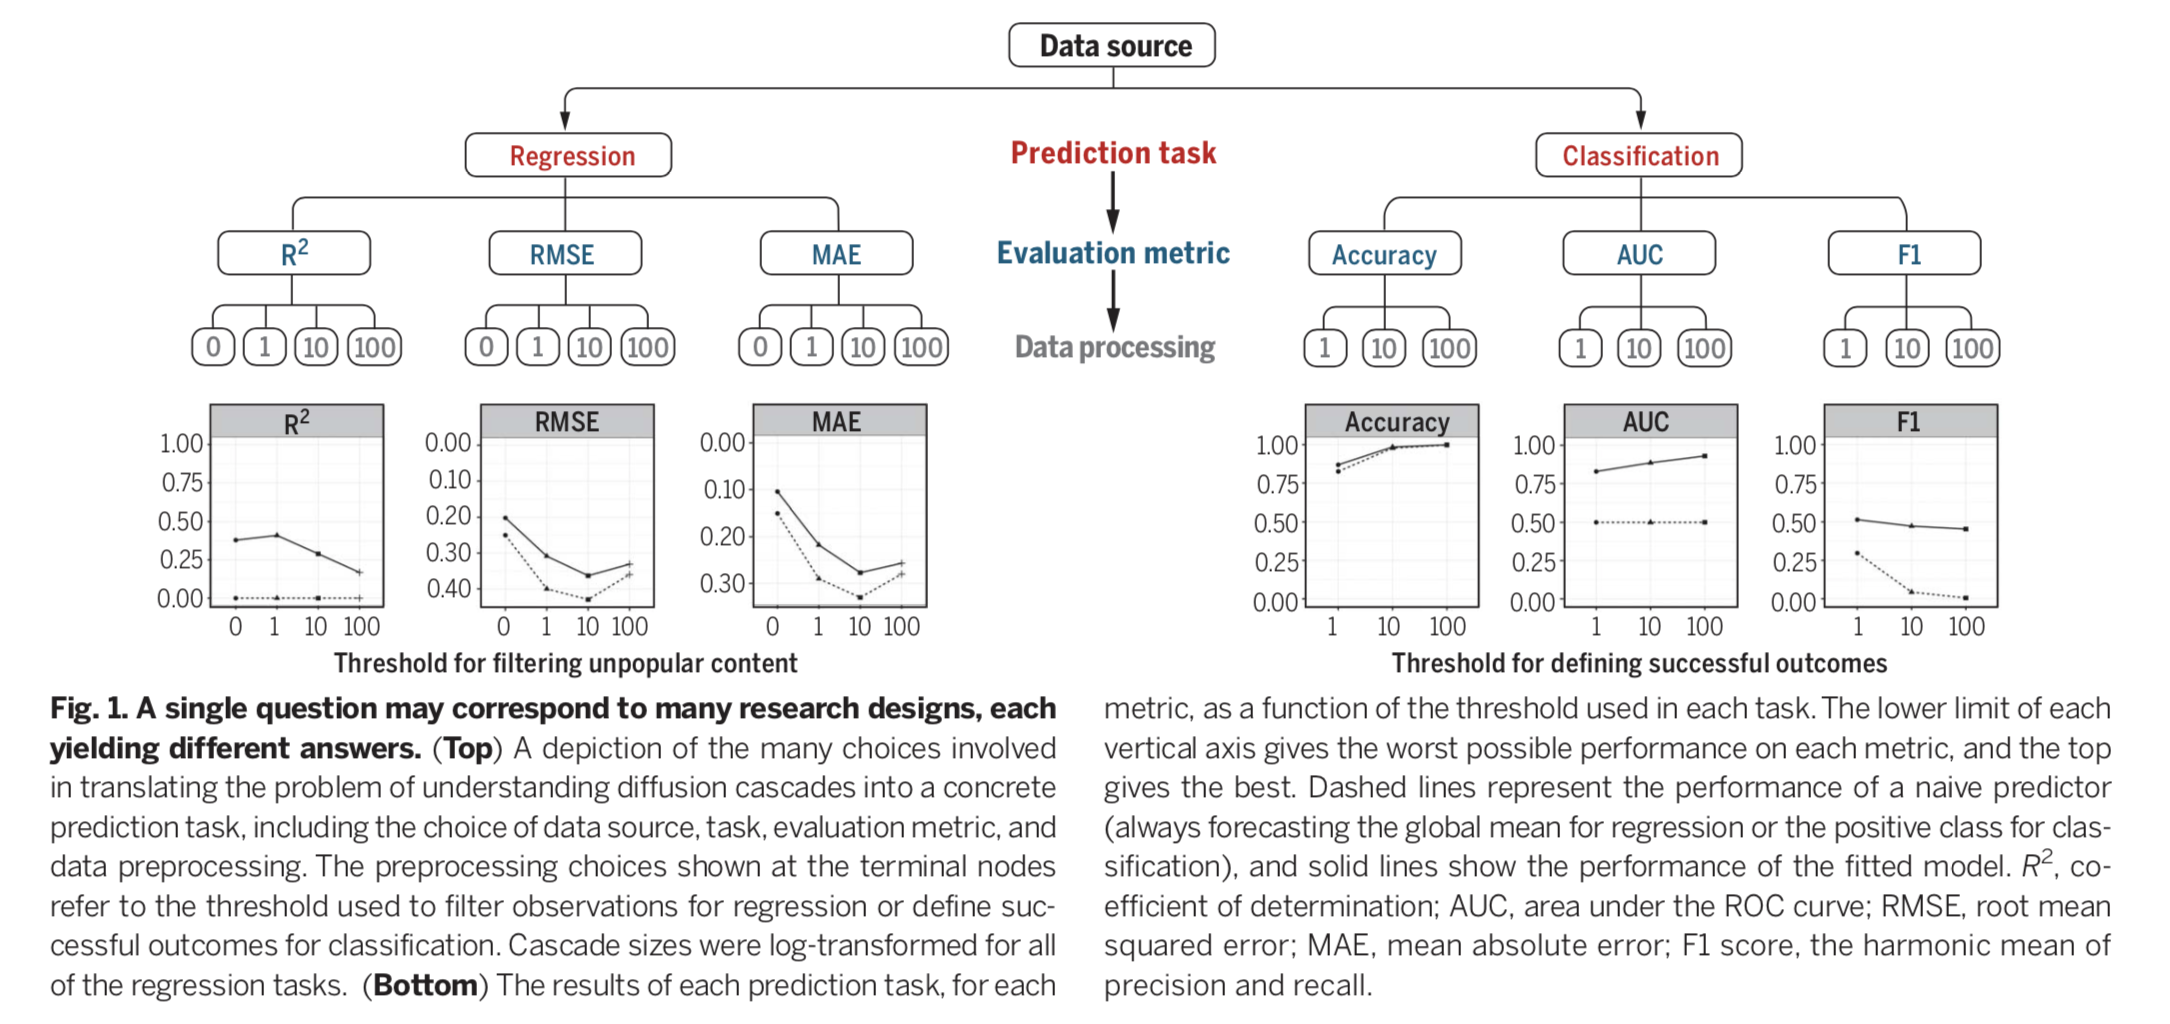
\includegraphics[width=0.9\textwidth]{figures/hofman_prediction_2017_fig1}
\end{center}

\vfill
This is why you have to pre-register assignment 1

\end{frame}
%%%%%%%%%%%%%%%%%%%%%%%%%%%%
\begin{frame}

\begin{center}
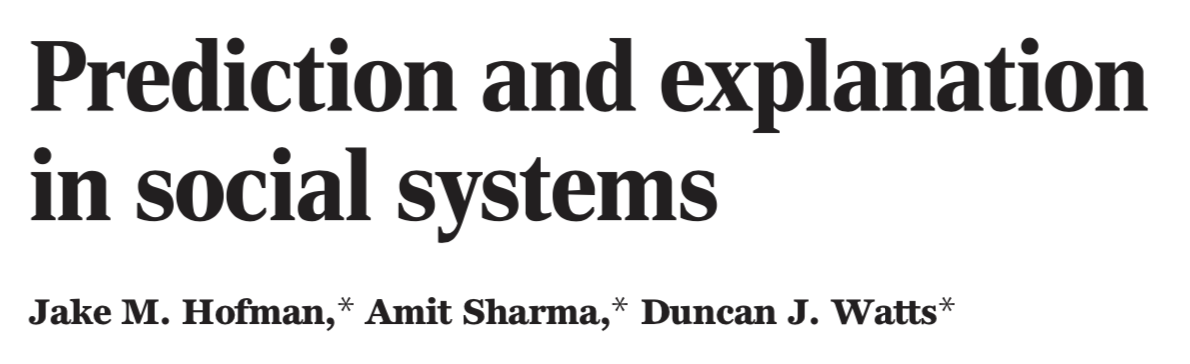
\includegraphics[width=0.9\textwidth]{figures/hofman_prediction_2017_title}
\end{center}

\end{frame}
%%%%%%%%%%%%%%%%%%%%%%%%%%%%%
\begin{frame}

Closing thoughts:
\begin{itemize}
\item social fads are partially unpredictable and partially predictable
\pause
\item likely mechanism is cumulative advantage
\pause
\item we see that same mechanism in other settings (e.g., disease)
\end{itemize}

\end{frame}
%%%%%%%%%%%%%%%%%%%%%%%%%%%%%


\frame{\titlepage}


\end{document}
